\chapter{KẾT QUẢ HIỆN THỰC VÀ ĐÁNH GIÁ}

Trong chương này, nhóm sẽ trình bày kết quả của việc hiện thực hai trong 3 module chính trong kiến trúc đề xuất ban đầu cho ứng dụng điều khiển cánh tay robot bằng kính VR, bao gồm khối phần cứng (máy tính RC5 + Cánh tay robot Denso VS-6577) và phần điều khiển bằng Ros2 với PC controller.

\section{Kết quả hiện thực}

\subsection{Kết quả demo}

Video demo của hệ thống điều khiển được trình bày tại đây: \href{https://drive.google.com/drive/folders/1OyP-rfXzVsNN-aHCGCSpOcyiajlx_tWP?usp=sharing}{Demo}

\subsection{Điều khiển Robot thông qua RC5}

Ở giai đoạn hai, đề tài đã tập trung cải thiện phương thức điều khiển bằng RC5, và hiện đã có một chu trình điều khiển ổn định và đáng tin cậy hơn rất nhiều so với giai đoạn trước đó. Nhờ việc phát hiện lỗi string đơn giản với CRC length, chương trình RC5 có thể chạy liên tục trong khoảng thời gian dài mà không bị lỗi gián đoạn. Với tốc độ truyền UART được set lên 119200 bit/s, thực nghiệm trong suốt quá trình phát triển cho thấy cứ 1000 lệnh gửi xuống RC5 sẽ có 2 lần lệnh bị lỗi, và chương trình RC5 hiện tại đã giúp loại bỏ vấn đề ngưng hệ thống mỗi khi chuỗi lệnh bị hỏng.

Khi việc xử lý chuỗi được ổn định, thì luồng thực thi để di chuyển cánh tay robot cũng ổn định theo. Với việc tách các hàm chạy theo chu kì, sử dụng ring buffer để tách biệt giữa luồng xử lý chuỗi và luồng thực thi, cánh tay robot có thể chạy với tốc độ cao hơn và nhanh hơn, trong khi vẫn đảm bảo an toàn và chương trình không bị gián đoạn.

\subsection{Hệ thống điều khiển với Ros2}

Dựa trên nền tảng Ros2, đề tài đã xây dựng và tích hợp thành công nhiều module khác nhau: hiện thực Ros2-control với Hardware interface và phần driver, protocol riêng biệt, cấu hình Ros2-controllers, cấu hình MoveIt2 tích hợp với Ros2-Control, tích hợp Gazebo cho mô phỏng thay thế Hardware Interface, sử dụng MoveIt-Servo, tạo custom Service Provider và Action Server, tích hợp RosBridge server cho giao tiếp Ros thông qua web socket. Hiện tại, dự án đang có đến 10 Ros-packages được sử dụng. Chi tiết về cách cài đặt có thể xem qua ở phần Readme của Repo: \href{https://github.com/ngoccatt/ros2_arctos_HCMUT/tree/cat_impl}{ros2\_arctos\_HCMUT}.

Sau khi đã clone repo và chuẩn bị hết tất cả những phụ thuộc môi trường (package ros-humble, python...), ta build dự án từ thư mục gốc bằng lệnh:

\begin{lstlisting}[style=bashstyle]
colcon build --symlink-install
\end{lstlisting}

Quá trình build sẽ diễn ra trong vài phút, và thực hiện build 10 module khác nhau như kết quả dưới:

\begin{lstlisting}[style=bashstyle]
colcon build --symlink-install
Starting >>> serial
Starting >>> denso_description
Starting >>> denso_interfaces
Starting >>> denso_moveit_servo
Starting >>> file_server2
Finished <<< denso_description [0.31s]
Starting >>> denso_moveit_config
Finished <<< serial [0.42s]
Starting >>> denso_motor_driver
Finished <<< denso_moveit_servo [0.42s]
Finished <<< denso_moveit_config [0.33s]
Finished <<< denso_motor_driver [0.39s]
Starting >>> denso_hardware_interface
Finished <<< file_server2 [1.37s]
Finished <<< denso_interfaces [1.41s]
Starting >>> denso_remote_control
Finished <<< denso_hardware_interface [0.83s]
Starting >>> denso_bringup
Finished <<< denso_remote_control [0.77s]
Finished <<< denso_bringup [1.64s]

Summary: 10 packages finished [4.25s]
\end{lstlisting}

Sau khi build thành công, ta "source" dự án để Ros2 biết được sự tồn tại của chương trình:

\begin{lstlisting}[style=bashstyle]
source install/setup.bash
\end{lstlisting}

Sau đó, ta có thể lần lượt chạy các module chính của dự án.

\subsubsection{Hệ thống điều khiển chính với Ros2-Control và MoveIt}

Để chạy chương trình điều khiển chính, người dùng gõ lệnh sau vào terminal

\begin{lstlisting}[style=bashstyle]
ros2 launch denso_bringup denso_bringup.launch.py use_sim_time:=false
\end{lstlisting}

File bringup có nhiệm vụ chạy hết tất cả các module liên quan, bao gồm:

\begin{itemize}
    \item Ros2-control manager
    \item Robot state publisher
    \item JointStateBoardcaster Ros2 Controller
    \item Denso\_arm\_controller
    \item Denso\_hand\_controller
    \item Rviz2
    \item MoveIt2 (MoveGroup)
    \item V4L2 camera node 1
    \item V4L2 camera node 2
\end{itemize}

Toàn bộ module Ros2-Control kèm controllers đều được khởi chạy, có sự tích hợp bởi MoveIt2 phía trên cho planning và Execution. Ngoài ra, các camera node cũng được khởi chạy để plublish các topic camera mà ứng dụng VR có thể sử dụng.

\textbf{Giao diện điều khiển cánh tay robot VS-6577 với Rviz}

Khởi chạy thành công, giao diện Rviz sẽ hiển thị ra như hình, bao gồm mô hình 3D của cánh tay và cả phần tay gắp. Lưu ý rằng mô hình tay gắp trong Rviz hiện tại không phản ánh chính xác hoạt động của của tay gắp, mà được đơn giản hóa hơn. Lý do là vì tay gắp thực tế có liên kết trục phức tạp và không thể xây dựng quan hệ một cha - một con trong URDF.

Trong Rviz, ta có thể thay đổi planning group để thay đổi đối tượng cần điều khiển. \textbf{denso\_arm} dùng để điều khiển sáu trục của cánh tay, còn \textbf{denso\_hand} dùng để điều khiển phần tay gắp. Velocity Scaling và Accel Scaling là tỉ lệ của vận tốc và gia tốc tối đa được cấu hình cho cánh tay. Hiện tại, đồ án nhận thấy Velocity scaling 0.4 cùng Accel. Scaling 0.3 đem lại hiệu quả điều khiển ổn định và mượt mà nhất.

\begin{figure}[H]
    \centering
    \begin{subfigure}{0.48\linewidth}
        \centering
        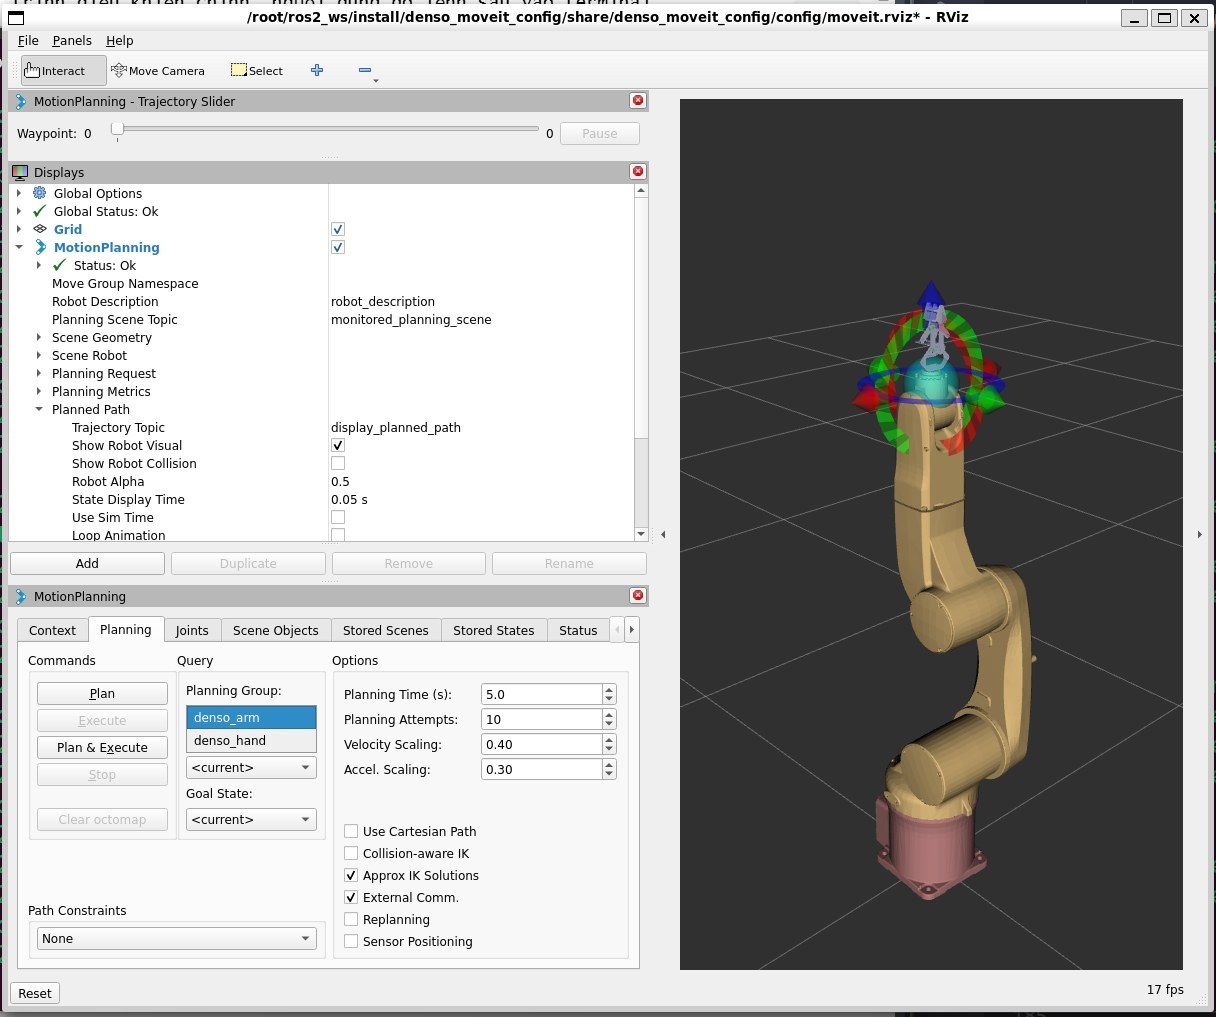
\includegraphics[width=\linewidth]{Images/Implementation/bringup1.jpg}
        \caption{Giao diện điều khiển chính với Rviz}
    \end{subfigure}
    \hfill
    \begin{subfigure}{0.48\linewidth}
        \centering
        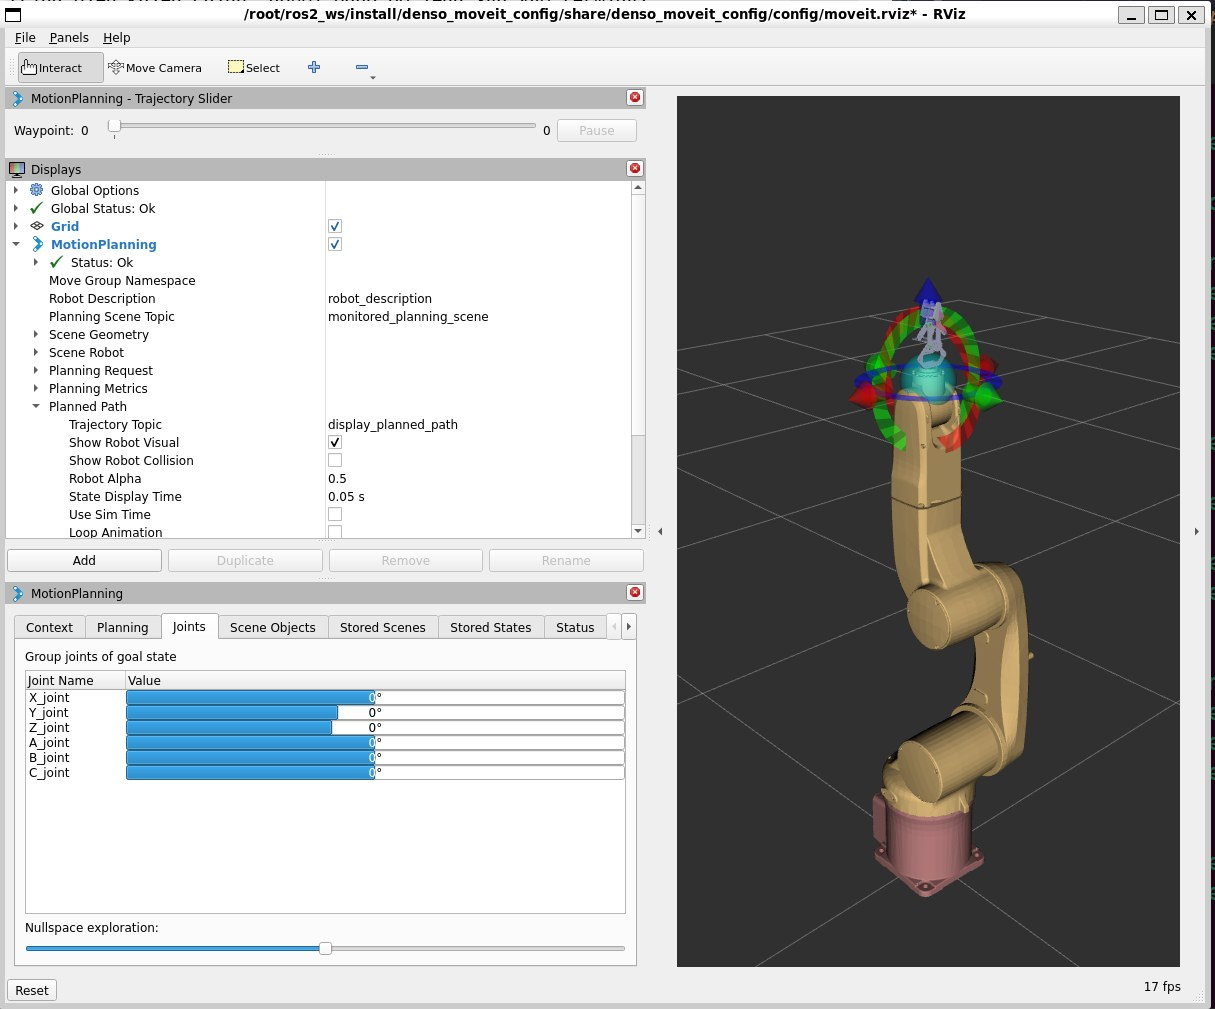
\includegraphics[width=\linewidth]{Images/Implementation/bringup2.jpg}
        \caption{Điều khiển các trục phần cánh tay}
    \end{subfigure}
    \hfill
    \begin{subfigure}{0.48\linewidth}
        \centering
        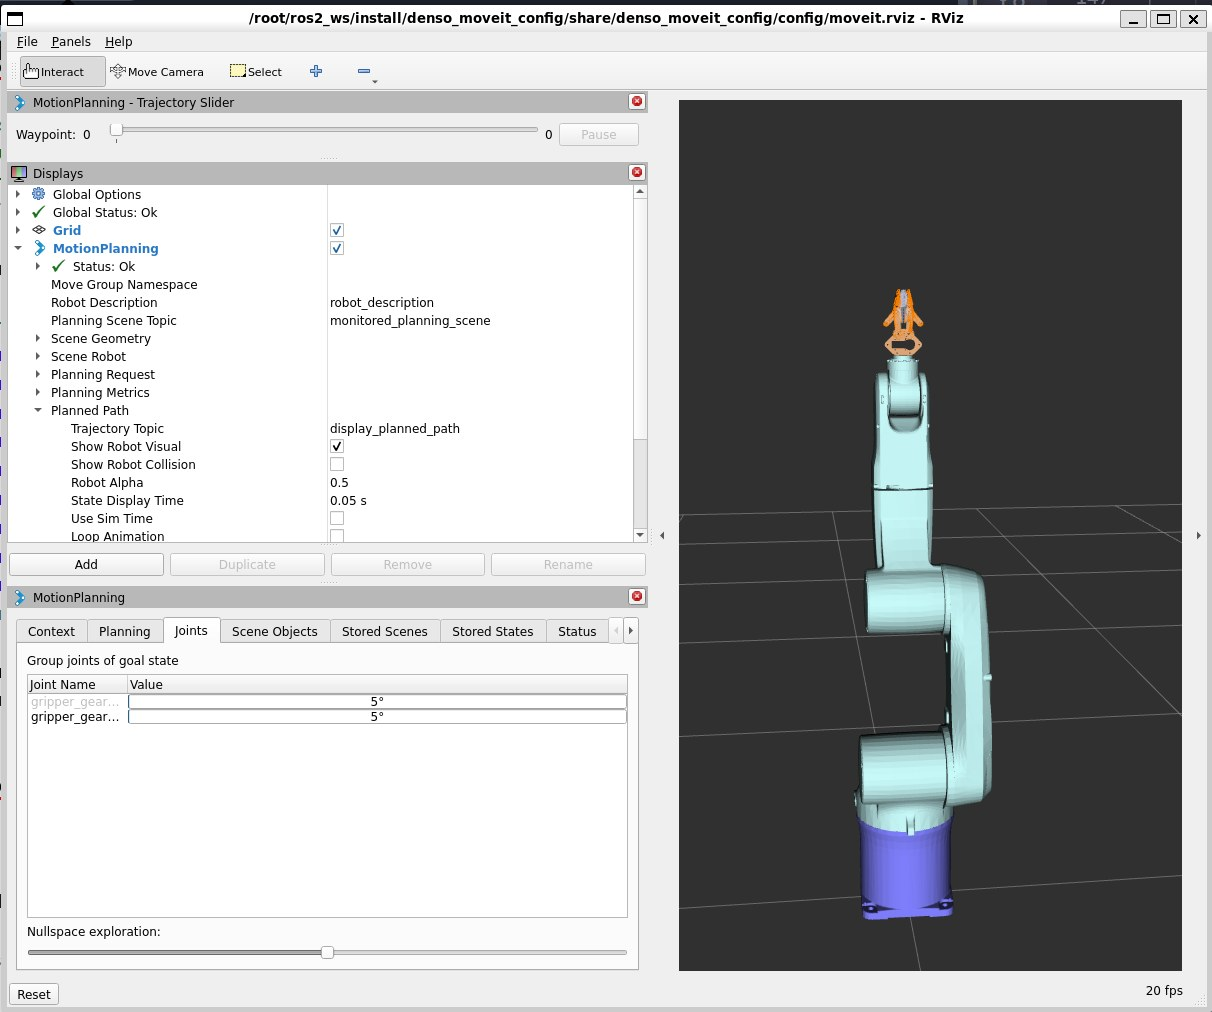
\includegraphics[width=\linewidth]{Images/Implementation/bringup3.jpg}
        \caption{Điều khiển các trục phần tay gắp}
    \end{subfigure}
    \caption{Kết quả khởi chạy hệ thống mô phỏng với Gazebo}
    \label{fig:eval-gazebo-bringup}
\end{figure}

Trong hộp thoại MotionPlanning, ở thẻ Joint, ta có thể tùy ý xoay từng trục cánh tay đích (goal state) để xem trạng thái của chúng. Các giá trị góc xoay sẽ được giới hạn, tuân theo thông tin được cấu hình ở file URDF hoặc các file cấu hình khác, nếu có. Khi cần điều khiển robot tương ứng, ta có thể chuyển qua tab Planning. Ở đây có hai chức năng: khi nhấn \textbf{Plan}, MoveIt sẽ thực hiện việc tính toán dựa theo thông tin về robot cũng như thuật toán động lực học đã chọn, và để xuất ra đường đi, hay quỹ đạo tối ưu để đưa robot từ vị trí hiện tại sang vị trí Goal. Lựa chọn \textbf{Execute} sẽ chỉ sáng lên sau khi planning hoàn tất, tức thực thi quá trình điều khiển để cánh tay thực tế có thể đi tới vị trí mục tiêu. Lựa chọn \textbf{Plan \& Execute} sẽ thực hiện tuần tự \textbf{Plan} và tự động \textbf{Execute} sau khi \textbf{Plan} hoàn tất.

Khi bấm \textbf{Execute}, Moveit sẽ bắt đầu gửi các trajectory tới Controller của cánh tay robot, và yêu cầu cánh tay robot quay dần để đạt tới vị trí đích. Từng giá trị Trajectory được truyền xuống Controller, tham gia vai trò của \textbf{update} trong chu kì ba bước. Sau \textbf{update}, các \lstinline[style=inlinecode]{command_interface} sẽ được ghi vào giá trị điều khiển, và \textbf{write} sử dụng các \lstinline[style=inlinecode]{command_interface}, tổng hợp thành một lệnh điều khiển đưa xuống máy RC5 theo định dạng phù hợp. Tiếp đó, \textbf{read} đọc trạng thái góc quay thực tế của cánh tay phản hồi từ RC5, cập nhật vào các \lstinline[style=inlinecode]{state_interface}. Giá trị trạng thái cũng được phản ánh ngay trên mô hình cánh tay Robot trên Rviz, và người dùng có thể thấy mô hình 3D mờ dần dần di chuyển tới vị trí đích.

\subsubsection{Hệ thống điều khiển mô phỏng với Ros2-Control, MoveIt2 và Gazebo}

Gazebo được tích hợp vào hệ thống để giúp cho việc phát triển ứng dụng nhanh chóng hơn, an toàn hơn nhờ môi trường mô phỏng, trước khi thử nghiệm trên cánh tay thực tế. Để chạy hệ thống điều khiển với Gazebo, chạy lện sau trong cửa sổ terminal:

\begin{lstlisting}[style=bashstyle]
ros2 launch denso_bringup gz_denso_bringup.launch.py use_sim_time:=true
\end{lstlisting}

So với file bringup cho thiết bị thực tế, gz\_denso\_bringup sẽ chạy các tác vụ sau:

\begin{itemize}
    \item Gazebo Sim (Ignition)
    \item Sinh mô hình robot trong Gazebo
    \item Cầu nối (bridge) giữa clock của Ros2 và clock của Gazebo
    \item JointStateBoardcaster Ros2 Controller
    \item Denso\_arm\_controller
    \item Denso\_hand\_controller
    \item Rviz2
    \item MoveIt2 (MoveGroup)
    \item V4L2 camera node 1
    \item V4L2 camera node 2
\end{itemize}

Ngoài việc chạy thêm các tác vụ liên quan tới Gazebo, lưu ý rằng Ros2-control manager đã không khởi chạy. Lý do là Gazebo khi được chọn là Hardware Interface thay thế (sử dụng gz\_ros2\_control::GazeboSimROS2ControlPlugin), nó sẽ tự chạy controller manager tự động, nên việc khởi chạy ros2-controol manager ở bringup là không cần thiết.

\begin{figure}[H]
    \centering
    \begin{subfigure}{0.48\linewidth}
        \centering
        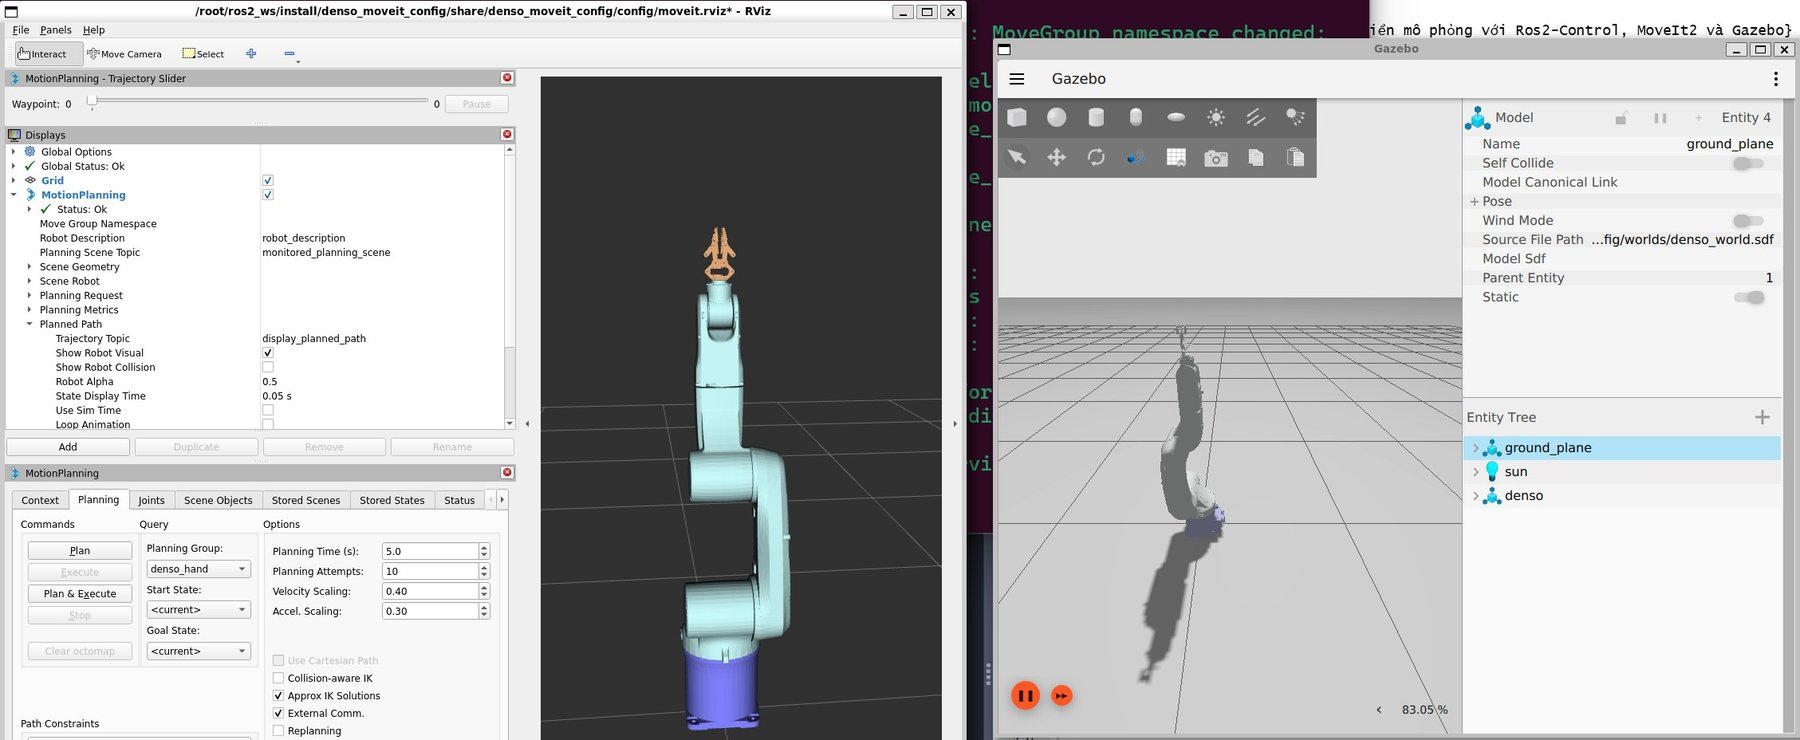
\includegraphics[width=\linewidth]{Images/Implementation/gz_bringup_1.jpg}
        \caption{Gazebo mô phỏng cánh tay robot}
    \end{subfigure}
    \hfill
    \begin{subfigure}{0.48\linewidth}
        \centering
        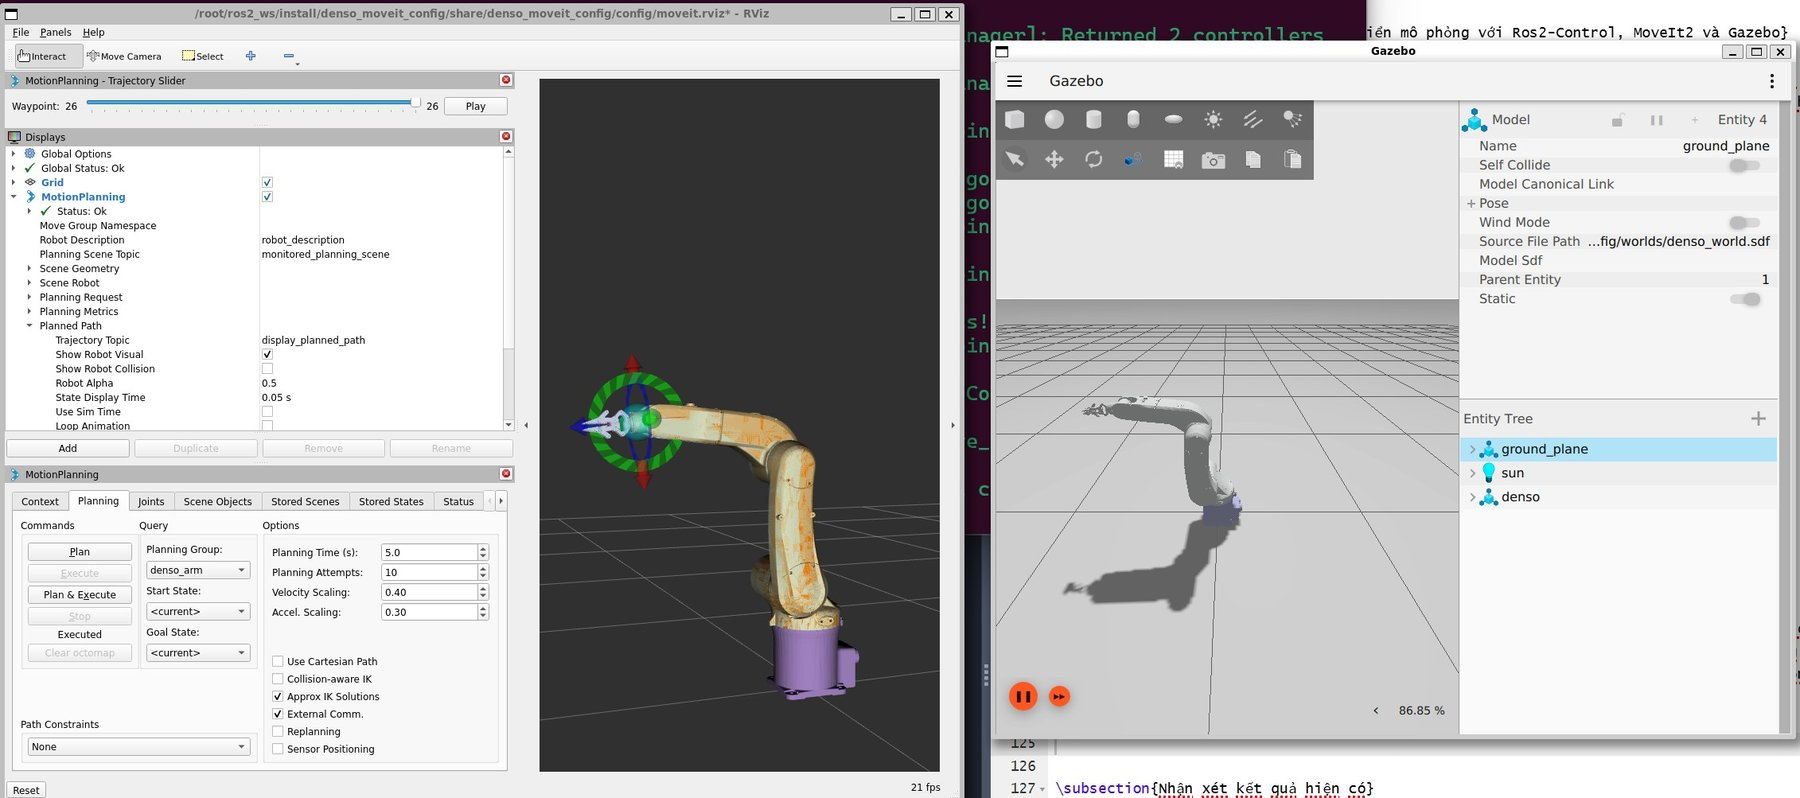
\includegraphics[width=\linewidth]{Images/Implementation/gz_bringup_2.jpg}
        \caption{Rviz đồng bộ với mô phỏng Gazebo}
    \end{subfigure}
    \caption{Kết quả khởi chạy hệ thống mô phỏng với Gazebo}
    \label{fig:eval-gazebo-bringup}
\end{figure}

Với hệ thống mô phỏng này, ta hoàn toàn có thể dùng Rviz để Planning, Execute các trục robot và điều khiển tay gắp mà không cần thiết bị thật, đồng thời thấy được phản hồi thay đổi trạng thái cánh tay khi Gazebo thực hiện thao tác di chuyển. Thêm nữa, ta sẽ không thể thực hiện kiểm thử module Hardware Interface do Gazebo đã thay thế module này trong vai trò thực hiện lệnh điều khiển và cập nhật trạng thái. Hệ thống mô phỏng sẽ chỉ hữu ích trong việc kiểm tra các tính năng từ tầng Hardware Interface trở lên: Các Controller, MoveIt và ứng dụng dựa trên MoveIt.

\subsubsection{Denso MoveIt-Servo Service provider}

Sau khi đã khởi chạy hệ thống chính, các module ứng dụng có thể lần lượt chạy để cung cấp phương thức điều khiển từ bên ngoài. Gõ lệnh sau vào terminal để chạy Denso Moveit-Servo:

\begin{lstlisting}[style=bashstyle]
ros2 launch denso_moveit_servo denso_moveit_servo.launch.py
\end{lstlisting}

Để có thể kiểm thử nhanh tính năng điều khiển với MoveIt Servo, ta có thể chạy thêm chương trình sau ở một terminal khác để xoay các trục robot bằng bàn phím:

\begin{lstlisting}[style=bashstyle]
ros2 run denso_moveit_servo servo_keyboard_input
\end{lstlisting}

\begin{figure}[H]
    \centering
    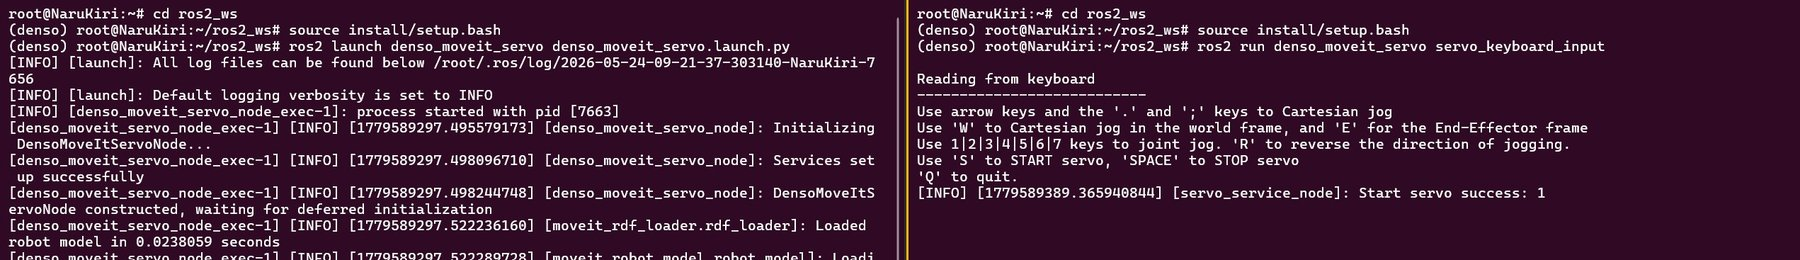
\includegraphics[width=0.9\linewidth]{Images/Implementation/denso_moveitservo.jpg}
    \caption{Node Denso MoveIt-Servo sau khi khởi chạy}
    \label{fig:eval-moveit-servo-node}
\end{figure}

\subsubsection{Denso Remote Control Action Server}

Tiếp theo, ta có thể chạy Action Server để nhận lệnh điều khiển Action dạng MoveToPose, để xoay robot tới vị trí yêu cầu. Ở một terminal khác, chạy lệnh sau:

\begin{lstlisting}[style=bashstyle]
ros2 launch denso_remote_control remote_control.launch.py
\end{lstlisting}

Ta có thể kiểm thử Action server này bằng việc gửi một Action Goal, với định dạng lệnh như sau (lưu ý phải source vào workspace trước khi sử dụng)

\begin{lstlisting}[style=bashstyle]
ros2 action send_goal /move_to_pose denso_interfaces/action/MoveToPose "{pose: {position: {x: 0.0, y: 0.0, z: 0.0}, orientation: {x: 0.0, y: 0.0, z: 0.0, w: 1.0}}, joints: [0.0, -0.5, 1.0, 0.0, 0.5, 0.0], use_pose: false}"
\end{lstlisting}

\begin{figure}[H]
    \centering
    \begin{subfigure}{0.48\linewidth}
        \centering
        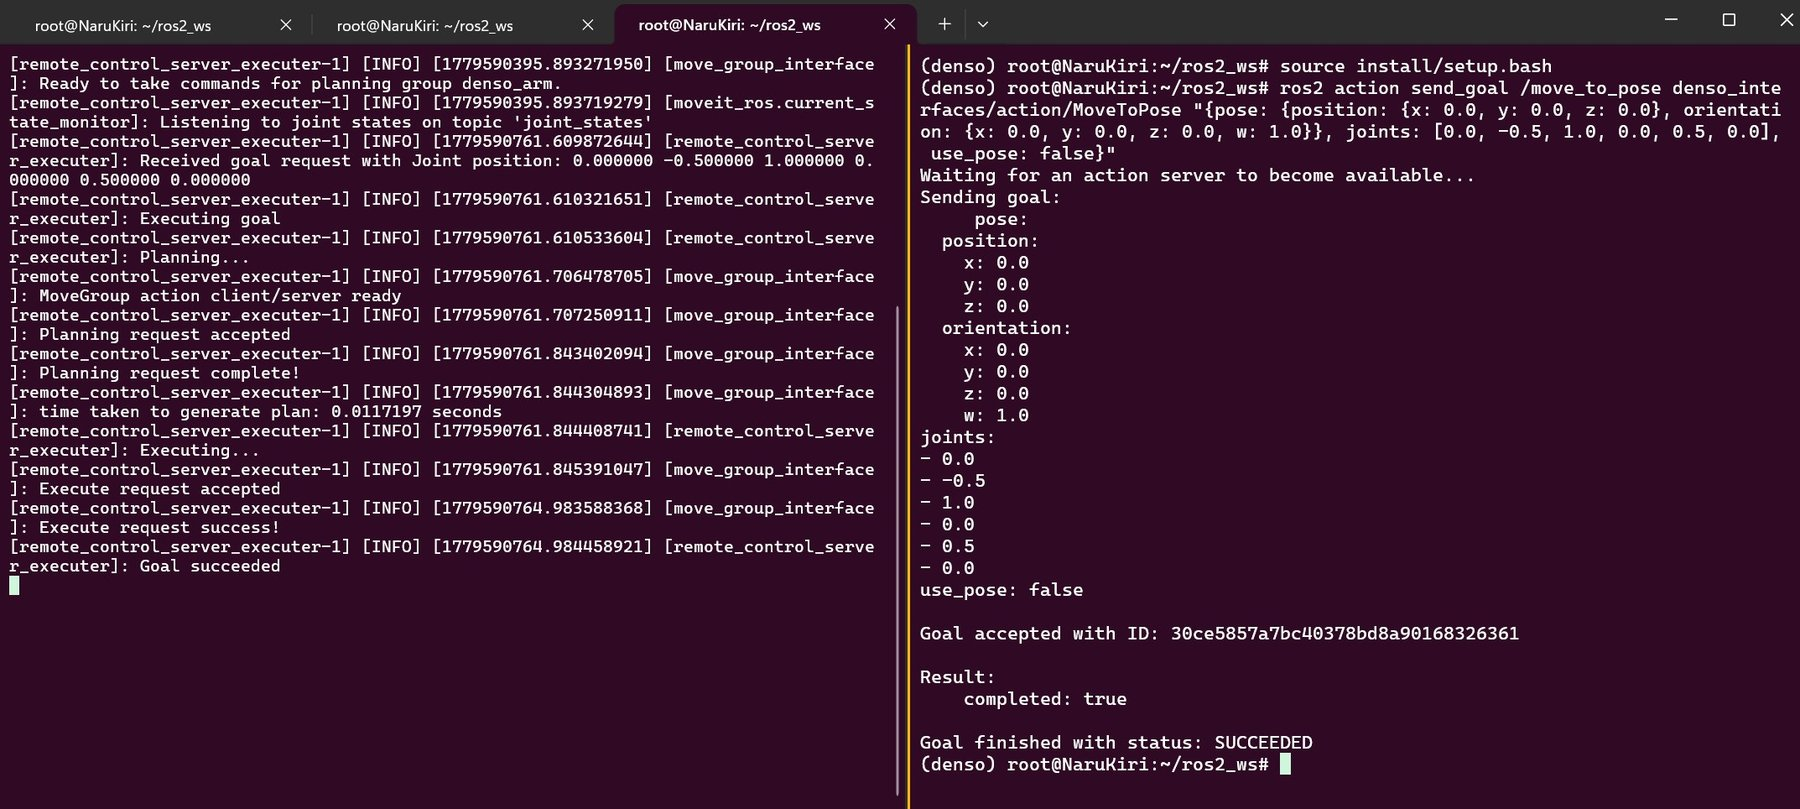
\includegraphics[width=\linewidth]{Images/Implementation/remote_control.jpg}
        \caption{Action Server Remote Control}
    \end{subfigure}
    \hfill
    \begin{subfigure}{0.48\linewidth}
        \centering
        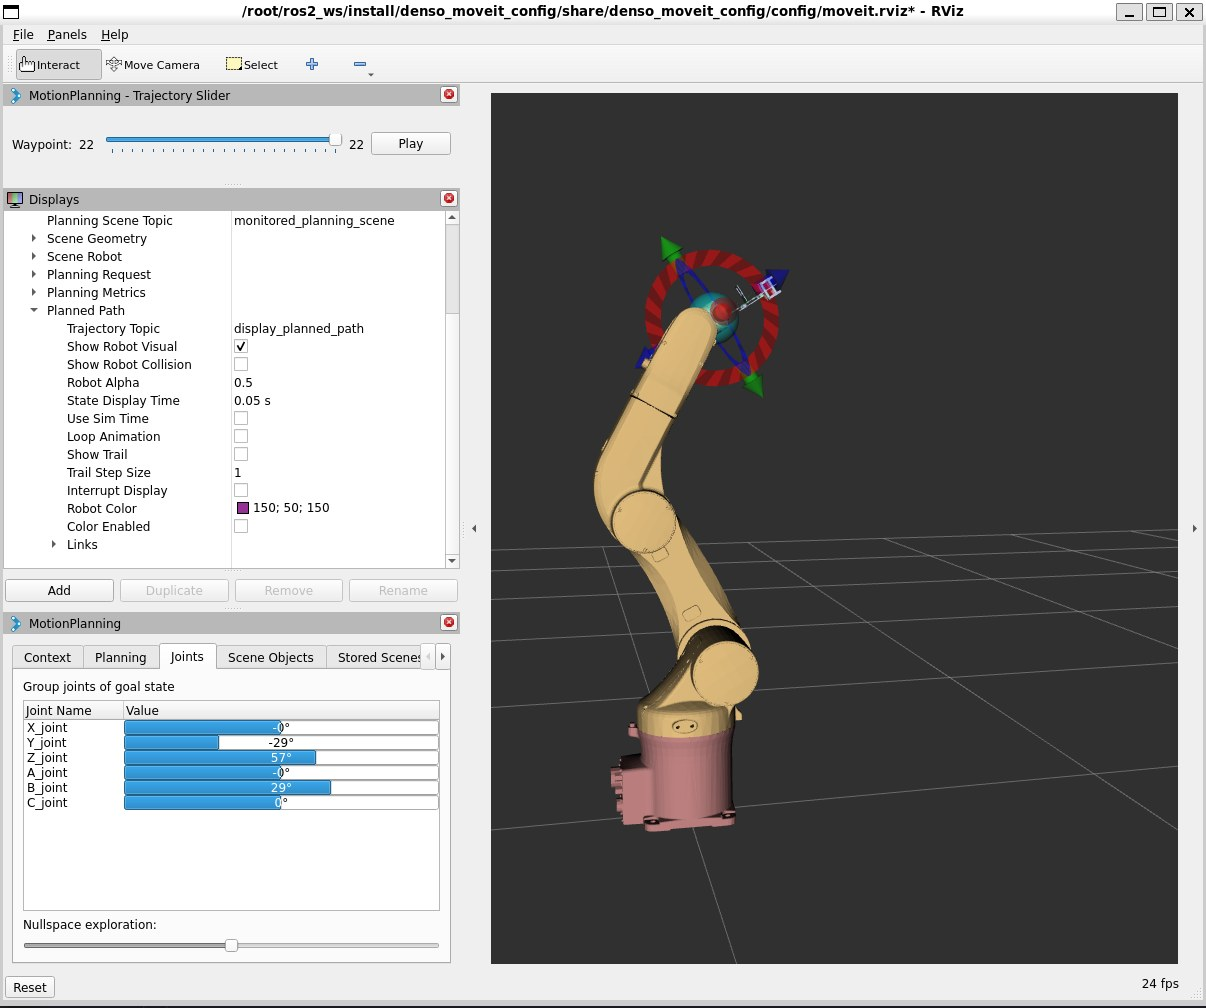
\includegraphics[width=\linewidth]{Images/Implementation/remote_control_1.jpg}
        \caption{Luồng phản hồi của Action Server}
    \end{subfigure}
    \caption{Kết quả kiểm thử Denso Remote Control}
    \label{fig:eval-remote-control}
\end{figure}

Lệnh trên thực hiện việc điều khiển robot bằng cách sử dụng danh sách giá trị các trục (theo đơn vị rad). Mô phỏng với Gazebo cho thấy robot đã xoay tới vị trí mong muốn.

\subsubsection{RosBridge Server}

Để có thể cho ứng dụng VR giao tiếp với Ros thông qua Web socket, ta cần chạy thêm RosBridge Server. Lệnh sau được sử dụng để chạy server cho kết nối:

\begin{lstlisting}[style=bashstyle]
ros2 launch file_server2 ros_sharp_communication.launch.py
\end{lstlisting}

\begin{figure}[H]
    \centering
    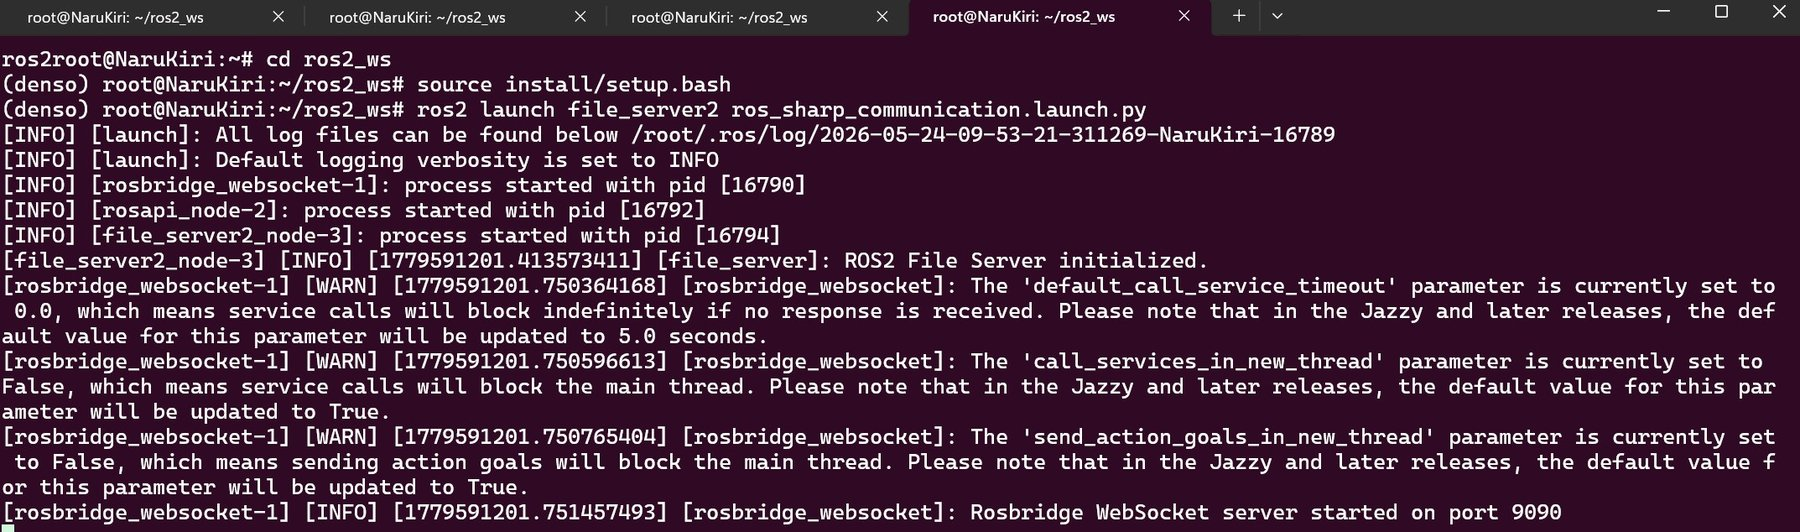
\includegraphics[width=0.90\linewidth]{Images/Implementation/rosbridge_server.jpg}
    \caption{RosBridge Server sẵn sàng kết nối cho ứng dụng VR}
    \label{fig:eval-rosbridge-server}
\end{figure}

RosBridge server được khởi chạy tại port 9090, cho phép ứng dụng Unity với Ros-Sharp có thể kết nối tới và sử dụng các topic/service/action tự do.

\subsubsection{Đánh giá về độ trễ Execution trên thiết bị thực tế}

Trong quá trình phát triển, đề tài nhận thấy rằng việc điều khiển cánh tay thực tế luôn có độ trễ: cánh tay robot cần xoay các motor để di chuyển, cần phải có quá trình gia tốc, giảm tốc, có ma sát và ảnh hưởng bởi trọng lực, nên giả định lý tưởng: "với một lệnh điều khiển, cánh tay robot sẽ xoay hoàn tất trước khi nhận lệnh tiếp theo" là khó để đạt được, ít nhất là với hệ thống hiện tại, khi Ros2-Control tính toán trước chuỗi trajectory và gửi lần lượt chuỗi đó theo chu kì cố định. Chính vì vậy, đề tài đã thực hiện nhiều lần kiểm thử để tìm một cấu hình tối ưu, nhằm đồng bộ nhất có thể giữa tần số điều khiển của Ros2 và thời gian hoạt động của cánh tay robot, gồm:

\begin{itemize}
    \item Cấu hình tốc độ tối đa của từng trục theo tài liệu kĩ thuật chính thức của cánh tay
    \item Sử dụng Velocity scaling và acceleration scaling gần tương đồng (nhỏ hơn) so với tốc độ của cánh tay ở RC5. Ví dụ, Velocity scaling là 0.4 thì tốc độ cánh tay sẽ là 46\%
    \item Lựa chọn tần số 10Hz cho hoạt động điều khiển của Ros2-Control, qua đó cho phép  hoạt động từ phía RC5 diễn ra trong 100ms với ba giai đoạn: Nhận lệnh UART (~10ms), Xử lý lệnh UART dạng chuỗi (20-30ms), Xoay cánh tay (60-70ms).
    \item Phản hồi trạng thái cánh tay từ RC5 lên Ros2 diễn ra mỗi 100ms, tương tự với chu kì điều khiển Ros2
\end{itemize}

"Độ trễ" được tính toán dựa trên mỗi lần planning với MoveIt2, là sai lệch kể từ lúc Ros2-control ngưng gửi lệnh xuống RC5 cho tới khi cánh tay robot hoàn thành hành động xoay. Bảng thống kê độ trễ từ hai phiên kiểm thử thực tế với tổng cộng 25 goals được trình bày dưới đây:

\begin{figure}[H]
\centering
\begin{tikzpicture}
\begin{axis}[
    width=0.92\linewidth,
    height=6.5cm,
    xlabel={Goal},
    ylabel={Thời gian (ms)},
    xmin=0.5, xmax=25.5,
    ymin=0, ymax=15000,
    xtick={1,2,...,25},
    xticklabel style={font=\scriptsize},
    yticklabel style={font=\small},
    ytick={0,2000,4000,6000,8000,10000,12000,14000},
    grid=both,
    grid style={line width=0.3pt, draw=gray!30},
    major grid style={line width=0.5pt, draw=gray!50},
    legend style={at={(0.98,0.98)}, anchor=north east, font=\small,
                  draw=gray!50, fill=white, row sep=1pt},
    legend cell align=left,
    tick align=outside,
    axis lines=left,
    scaled ticks=false,
]
% T_tong
\addplot[color=blue!70, mark=square*, mark size=2pt, line width=1.2pt]
coordinates {
    (1,5797)(2,7898)(3,3396)(4,5698)
    (5,6698)(6,7698)(7,6296)(8,3699)(9,13798)(10,5699)
    (11,5799)(12,6198)(13,9399)(14,4799)(15,6898)(16,4898)
    (17,1699)(18,3199)(19,1599)(20,1299)(21,2199)
    (22,5698)(23,7098)(24,4399)(25,9499)
};
\addlegendentry{$T_\text{tổng}$}
% T_gui
\addplot[color=teal, mark=triangle*, mark size=2.5pt, line width=1.2pt, dashed]
coordinates {
    (1,3698)(2,6598)(3,1497)(4,3700)
    (5,3699)(6,5799)(7,5797)(8,1599)(9,10199)(10,3099)
    (11,3099)(12,4399)(13,5799)(14,3099)(15,5098)(16,2498)
    (17,899)(18,1099)(19,899)(20,599)(21,600)
    (22,2999)(23,5299)(24,1999)(25,5899)
};
\addlegendentry{$T_\text{gửi}$}
% T_dung
\addplot[color=red!80, mark=*, mark size=2.5pt, line width=1.5pt]
coordinates {
    (1,2099)(2,1300)(3,1899)(4,1999)
    (5,2999)(6,1899)(7,499)(8,2100)(9,3600)(10,2599)
    (11,2700)(12,1800)(13,3600)(14,1699)(15,1800)(16,2399)
    (17,800)(18,2099)(19,700)(20,700)(21,1599)
    (22,2699)(23,1800)(24,2400)(25,3599)
};
\addlegendentry{$T_\text{dừng}$ (độ trễ vật lý)}
% Duong trung binh T_dung
\addplot[color=red!80, line width=0.8pt, dotted, domain=0.5:25.5] {2055};
\addlegendentry{$\overline{T_\text{dừng}}$ = 2055\,ms}
\end{axis}
\end{tikzpicture}
\caption{Biểu đồ độ trễ Execution theo từng goal -- đường đỏ ($T_\text{dừng}$) là độ trễ vật lý sau khi Ros2 ngừng gửi lệnh}
\label{fig:moveit-latency-chart}
\end{figure}

\begin{table}[H]
\centering
\caption{Thống kê tổng hợp độ trễ Execution của MoveIt2 ($N = 25$ goals)}
\label{tab:moveit-execution-latency}
\begin{tblr}{
    colspec = {|X[3.5,l]|X[1.2,c]|X[1.2,c]|X[1.4,c]|X[1.2,c]|},
    hlines,
    row{1} = {font=\bfseries, bg=gray!20},
}
Chỉ số & Min (ms) & TB (ms) & Trung vị (ms) & Max (ms) \\
$T_\text{gửi}$ (\texttt{goal\_to\_last\_write}) & 599 & 3599 & 3099 & 10199 \\
$T_\text{dừng}$ (\texttt{last\_write\_to\_settle}) & 499 & 2055 & 1999 & 3600 \\
$T_\text{tổng}$ (\texttt{goal\_to\_settle}) & 1299 & 5654 & 5699 & 13798 \\
\end{tblr}
\end{table}

Tiêu chí đánh giá trọng tâm là $T_\text{dừng}$ -- khoảng thời gian sau khi MoveIt2 ngừng gửi lệnh mà cánh tay vẫn tiếp tục di chuyển do quán tính cơ học. Đây là giai đoạn Ros2 không còn can thiệp nhưng robot chưa dừng hẳn, thể hiện trực tiếp độ lệch giữa trạng thái điều khiển phần mềm và trạng thái vật lý của cánh tay.

$T_\text{dừng}$ đo được trung bình \textbf{2055\,ms} (trung vị 1999\,ms), dao động từ 499\,ms đến 3600\,ms. Đáng chú ý là $T_\text{dừng}$ ít phụ thuộc vào độ dài quỹ đạo hơn $T_\text{gửi}$: ngay cả với các chuyển động nhỏ (goals 17, 19, 20 -- $T_\text{gửi}$ chỉ 599–899\,ms), $T_\text{dừng}$ vẫn đạt 700–800\,ms, phản ánh thời gian giảm tốc tối thiểu cần thiết để cơ cấu dừng hoàn toàn. Với chuyển động lớn hơn, $T_\text{dừng}$ tăng lên 2000–3600\,ms do động năng cơ học tích lũy lớn hơn.

$T_\text{gửi}$ trung bình \textbf{3599\,ms} ($\approx$\,64\% tổng thời gian) tương đương khoảng 36 bước waypoints tại 10\,Hz. Giá trị này phụ thuộc trực tiếp vào độ phức tạp của quỹ đạo: goal~9 (ngoại lệ, nền vàng) có $T_\text{gửi}$ = 10199\,ms ($\approx$\,102 waypoints) do nhiều bậc tự do đồng thời di chuyển góc lớn, dẫn đến $T_\text{tổng}$ = 13798\,ms.

Nhìn chung, $T_\text{tổng}$ trung bình \textbf{5654\,ms} (trung vị 5699\,ms) là tổng hợp của cả hai giai đoạn. Với cấu hình Velocity scaling 0.4 -- Accel. scaling 0.3 và chu kỳ điều khiển 100\,ms, $T_\text{dừng}$ $\approx$\,2\,s là mức độ trễ vật lý cần chấp nhận trong ứng dụng điều khiển từ kính VR: sau khi thao tác, người dùng cần chờ khoảng 2\,s để cánh tay dừng hoàn toàn và sẵn sàng nhận lệnh tiếp theo.

\subsection{Ứng dụng VR điều khiển cánh tay robot}

Ứng dụng VR được xây dựng thành công và hầu như không có bất kì xung đột package nào - ứng dụng có thể được build thành một file cài đặt và chạy độc lập trên kính VR Meta Quest 3. Các tính năng của ứng dụng cho phép người dùng tự do lựa chọn phương thức điều khiển cánh tay robot và việc điều khiển có tính ổn định, đồng bộ cao với cánh tay thực tế thông qua giao tiếp Ros-sharp. 

\subsubsection{Các tính năng của ứng dụng}

Các tính năng được hỗ trợ bởi ứng dụng bao gồm:

\textbf{Kết nối/ Ngắt kết nối với Ros2 sử dụng địa chỉ IP và port}

\begin{figure}[H]
    \centering
    \begin{subfigure}{0.48\linewidth}
        \centering
        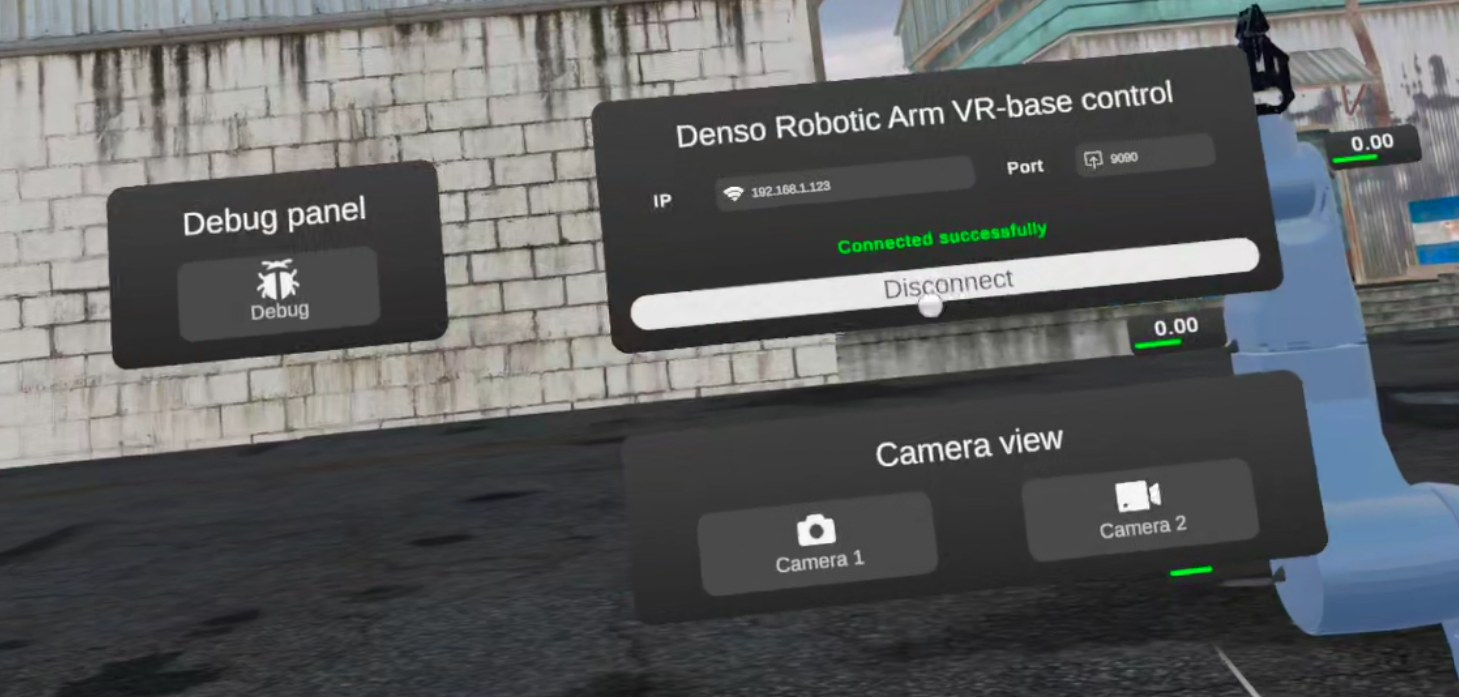
\includegraphics[width=\linewidth]{Images/Implementation/vr_connect.jpg}
        \caption{Trạng thái đã kết nối}
    \end{subfigure}
    \hfill
    \begin{subfigure}{0.48\linewidth}
        \centering
        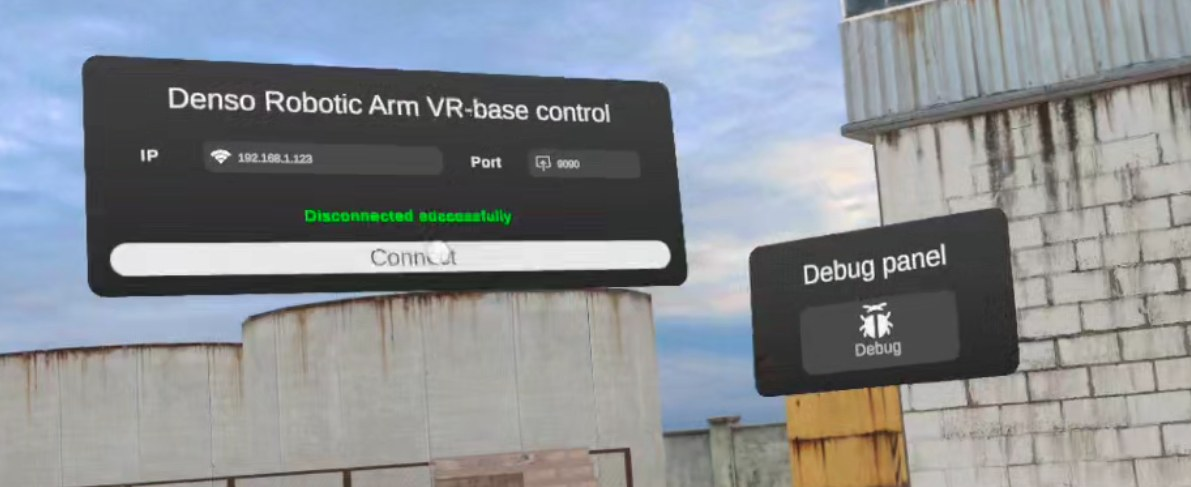
\includegraphics[width=\linewidth]{Images/Implementation/vr_disconnect.jpg}
        \caption{Trạng thái ngắt kết nối}
    \end{subfigure}
    \caption{Giao diện kết nối Ros2 trong ứng dụng VR}
    \label{fig:eval-vr-connect-disconnect}
\end{figure}

Khi kết nối thành công, các module và bảng điều khiển khác sẽ hiện ra để người dùng điều khiển robot. Thêm nữa, mọi bảng điều khiển trong ứng dụng để có thể tương tác và nắm được, nên người dùng cũng có thể tự do sắp xếp các bảng điều khiển trong môi trường cho tiện sử dụng.

\textbf{Bật/Tắt hai camera môi trường để quan sát}

Sau khi kết nối, người dùng có thể nhấn vào nút Camera 1 / Camera 2 để mở màn hình video xem dữ liệu truyền từ camera thông qua Ros2 topic. Debug panell được cung cấp kèm theo cho mục đích debug.

\begin{figure}[H]
    \centering
    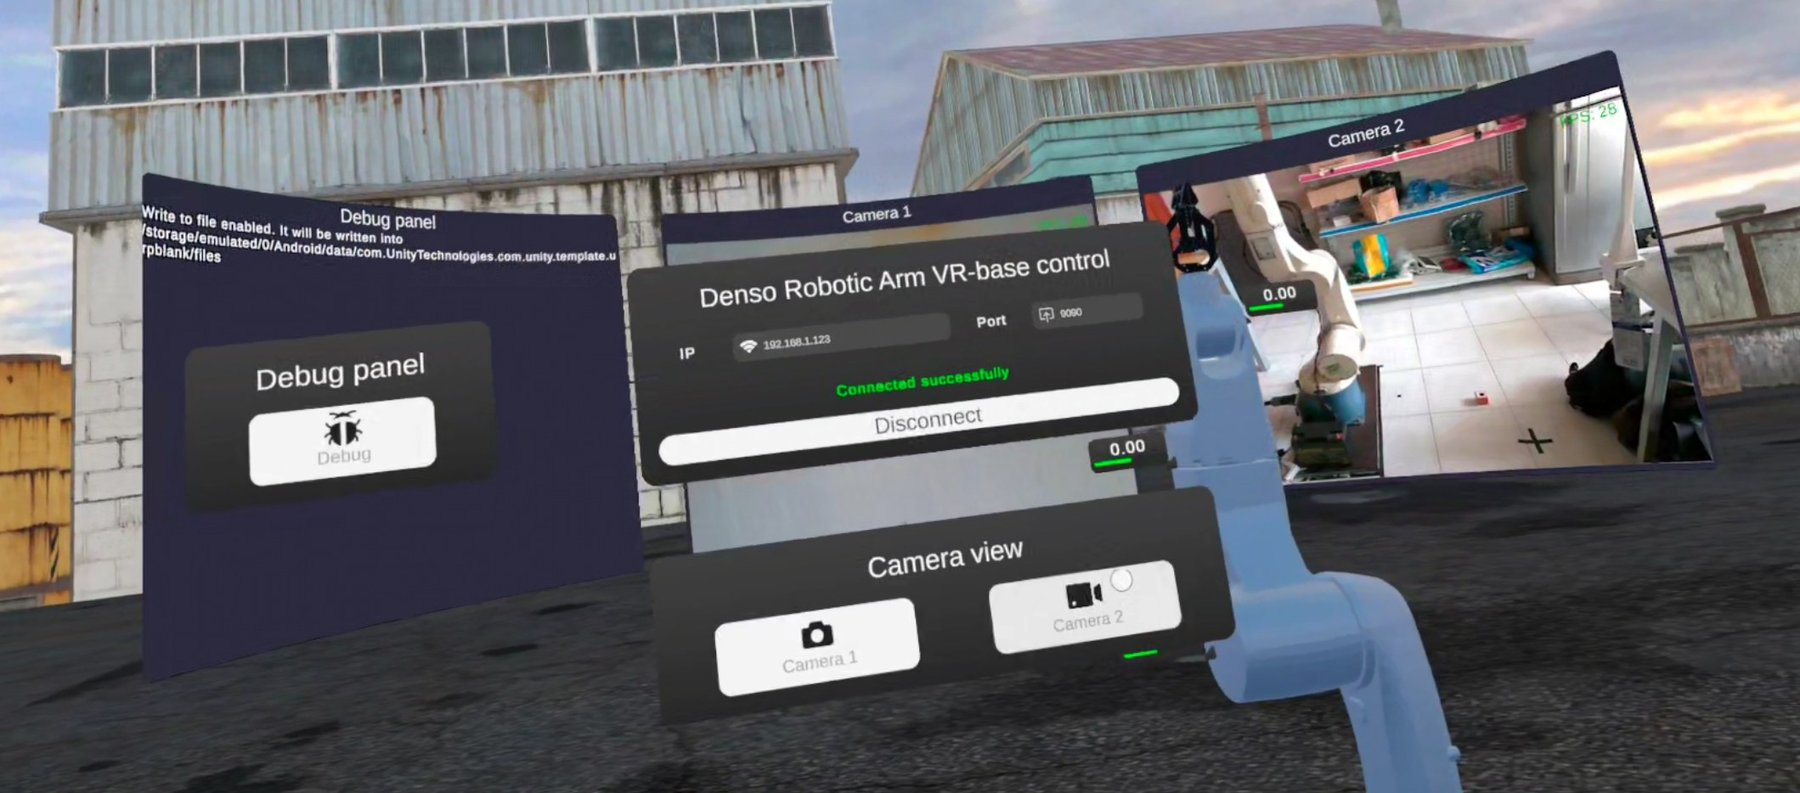
\includegraphics[width=0.8\linewidth]{Images/Implementation/vr_camera.jpg}
    \caption{Hiển thị hai luồng camera trong ứng dụng VR}
    \label{fig:eval-vr-camera}
\end{figure}

\textbf{Điều khiển bằng MoveIt-Servo}

Bảng điều khiển cho phép xoay các trục của cánh tay robot thực tế bằng nút "+" hoặc "-" ở hai bên hàng. Ở giữa hàng, giá trị số cho biết góc của trục tương ứng (đơn vị độ).

\begin{figure}[H]
    \centering
    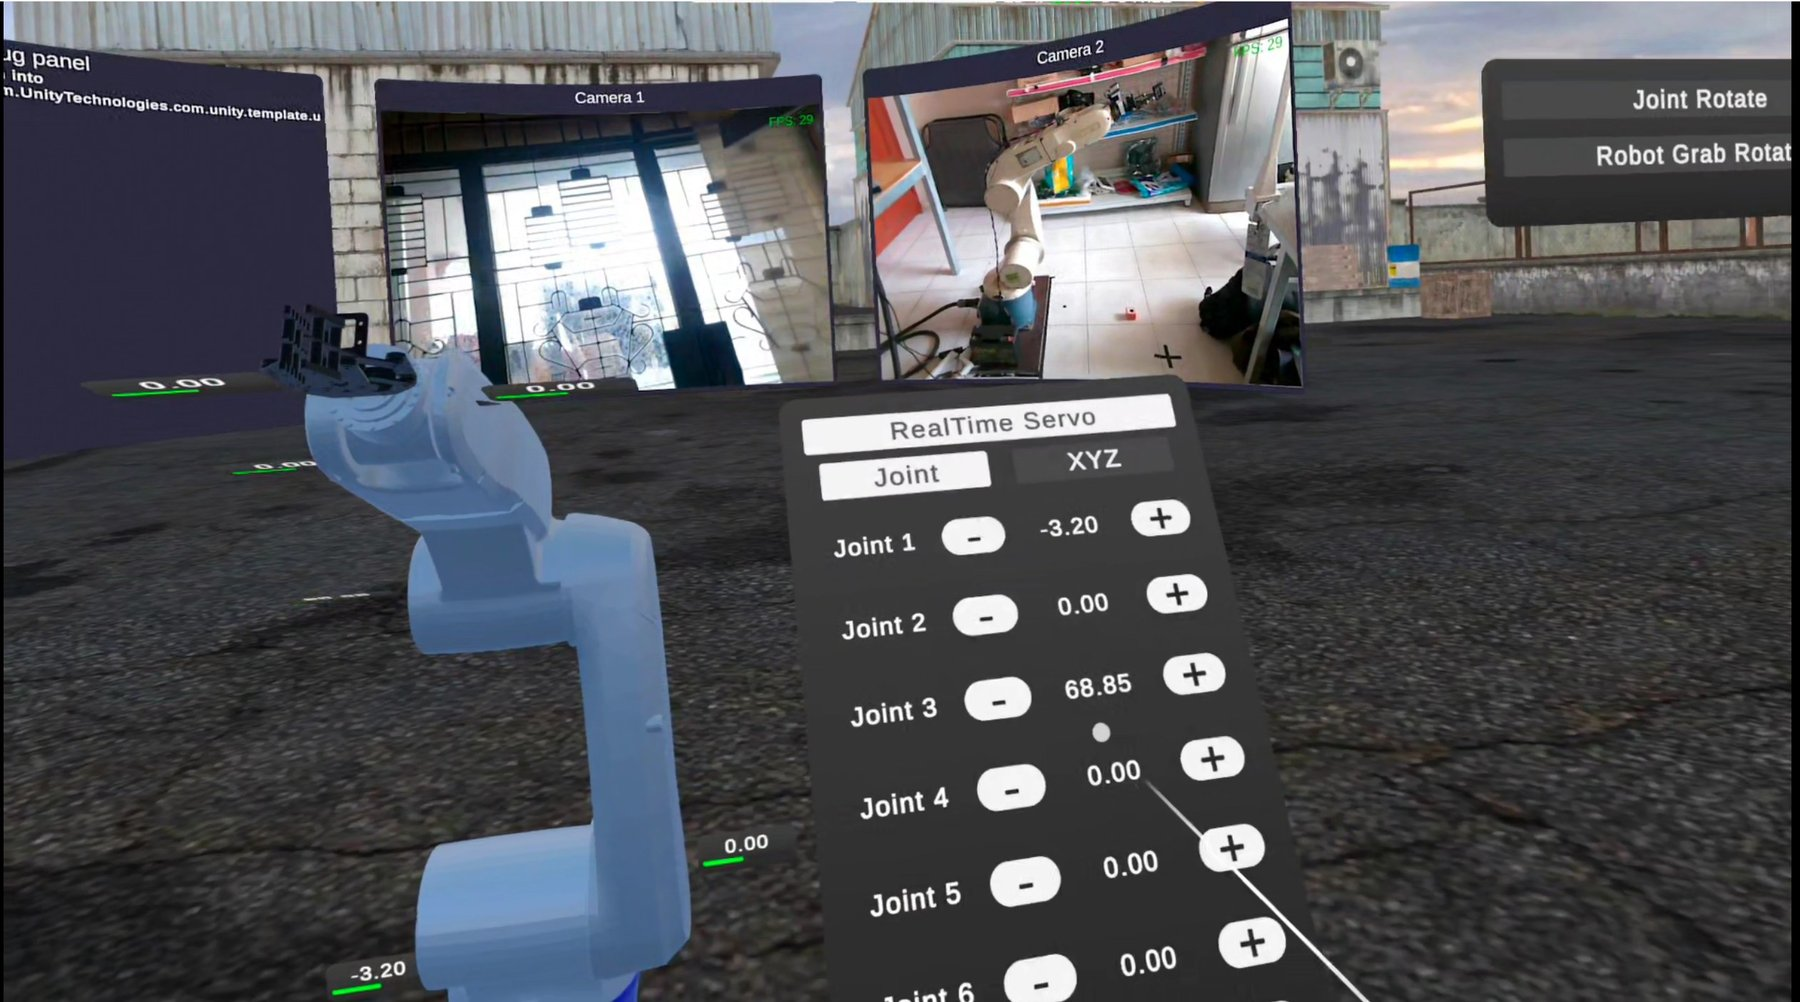
\includegraphics[width=0.8\linewidth]{Images/Implementation/vr_moveit_servo.jpg}
    \caption{Bảng điều khiển MoveIt-Servo trong ứng dụng VR}
    \label{fig:eval-vr-moveit-servo}
\end{figure}

\textbf{Điều khiển tay gắp với GripperCommand Action}

Việc điều khiển tay gắp được tích hợp trên bảng điều khiển MoveIt-Servo do nó cũng điều khiển thiết bị thực tế trực tiếp và đơn giản. Nút nhấn "Close" và "Open" gửi lệnh để đóng hoặc mở phần tay gắp. Trạng thái tay gắp thực tế được phản hồi qua chính mô hình 3D Denso Robot.

\begin{figure}[H]
    \centering
    \begin{subfigure}{0.48\linewidth}
        \centering
        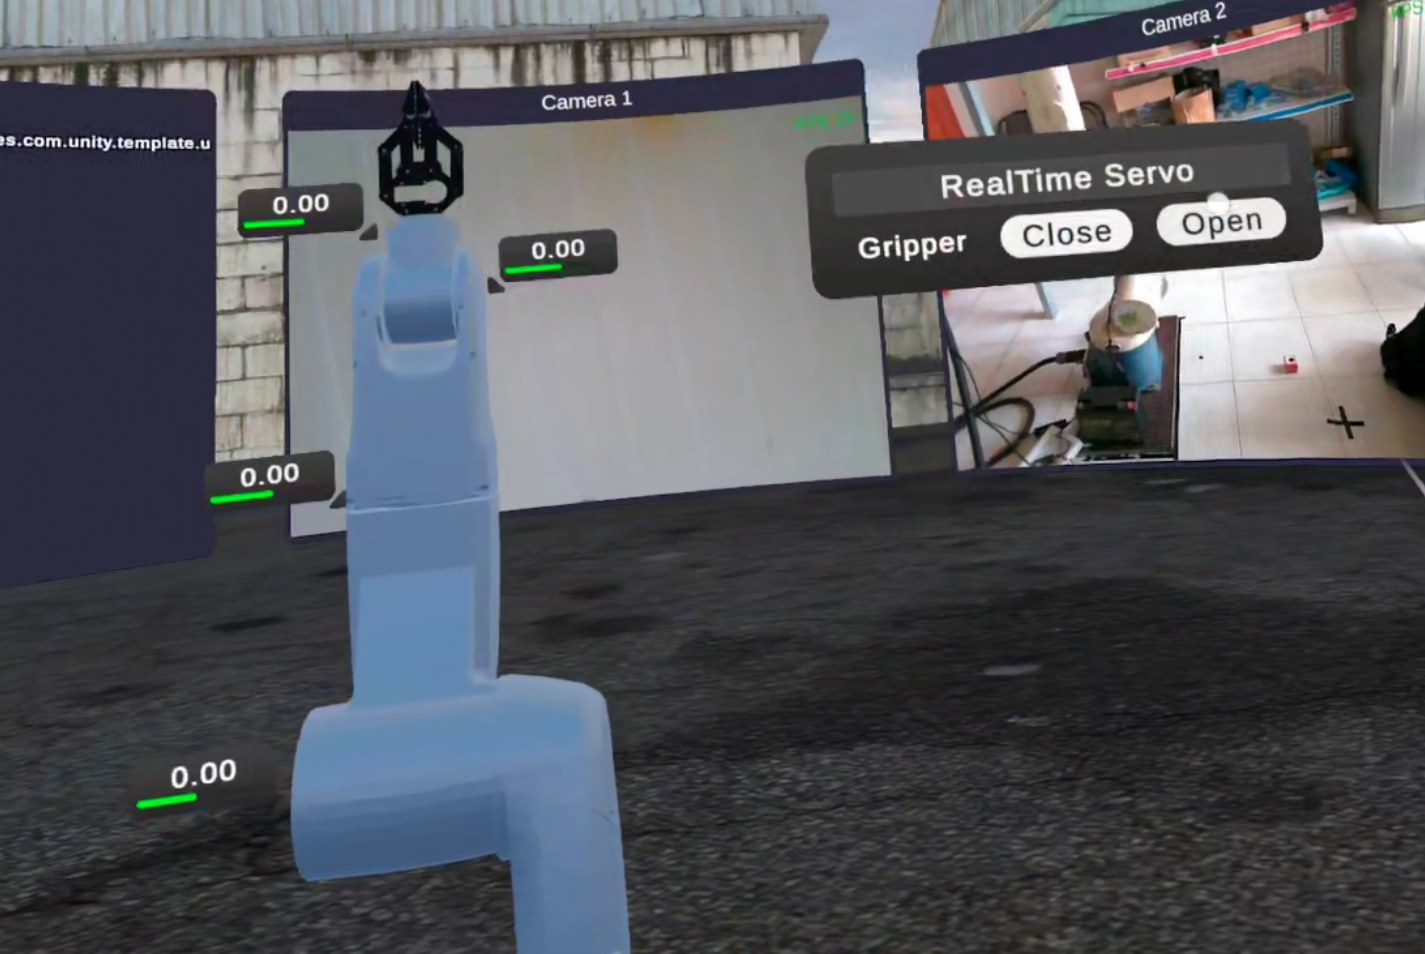
\includegraphics[width=\linewidth]{Images/Implementation/vr_gripper_open.jpg}
        \caption{Tay gắp ở trạng thái đóng}
    \end{subfigure}
    \hfill
    \begin{subfigure}{0.48\linewidth}
        \centering
        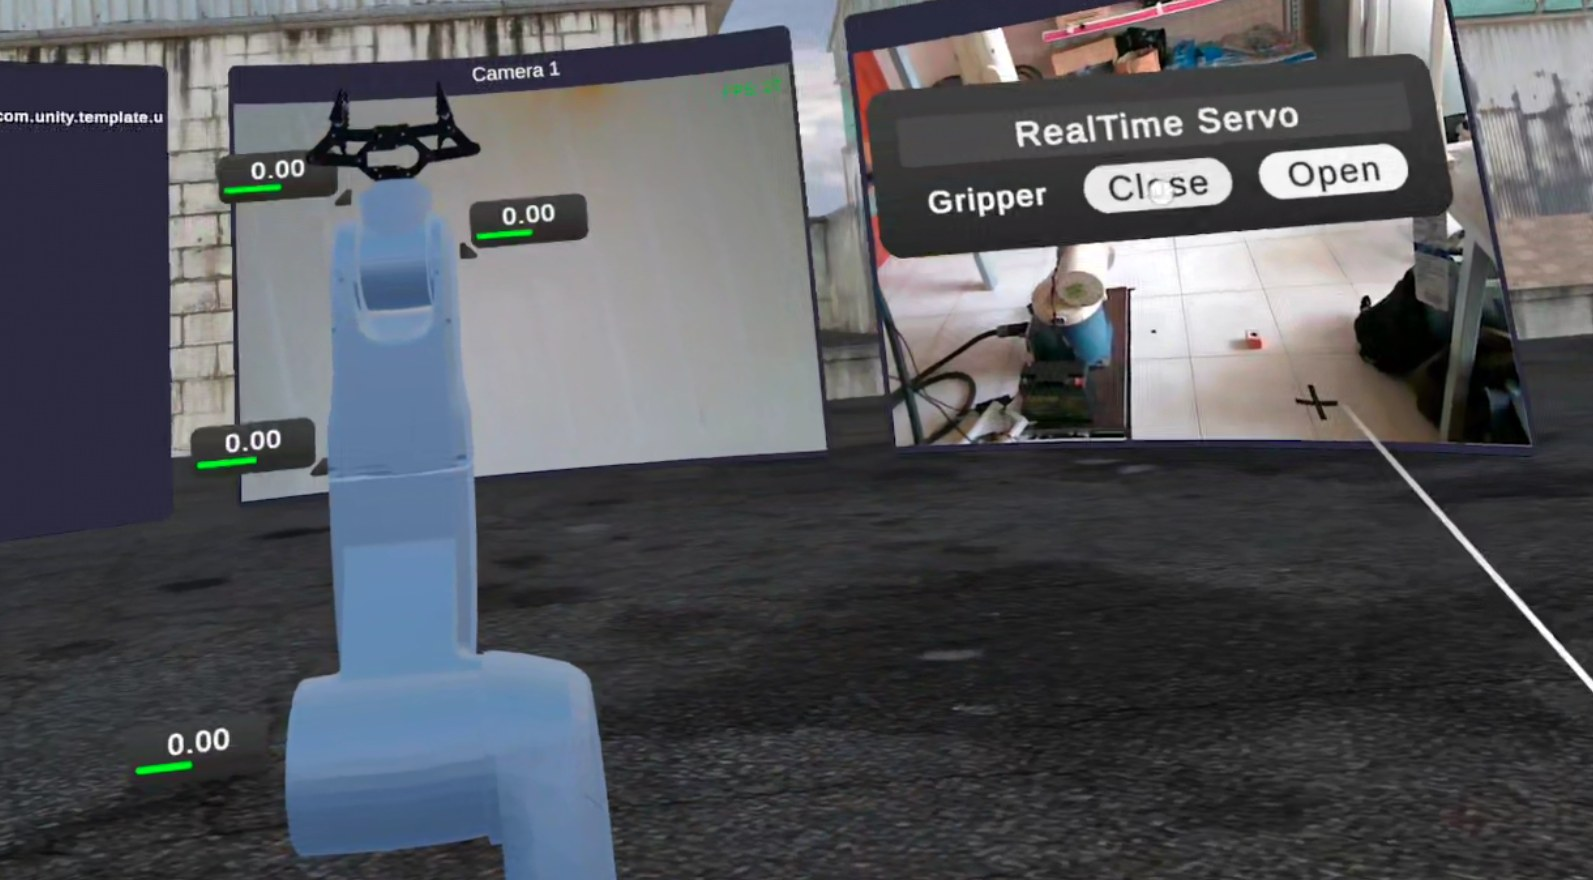
\includegraphics[width=\linewidth]{Images/Implementation/vr_gripper_close.jpg}
        \caption{Tay gắp ở trạng thái mở}
    \end{subfigure}
    \caption{Điều khiển tay gắp bằng GripperCommand Action}
    \label{fig:eval-vr-gripper}
\end{figure}

\textbf{Điều khiển cánh tay robot thông qua các Slider trên bảng điều khiển}

Nhấn vào nút Joint Rotate để chuyển sang bảng điều khiển bằng Slider. Khi này, một robot thứ hai sẽ xuất hiện, và xoay các trục theo giá trị của slider, nhằm cho người dùng biết cánh tay sẽ ở trạng thái như thế nào ở các vị trí tương ứng. Nhấn nút Execute sẽ gửi lệnh tới MoveToPose action server, nhằm điều khiển cánh tay thực tế đạt đến vị trí mong muốn.

\begin{figure}[H]
    \centering
    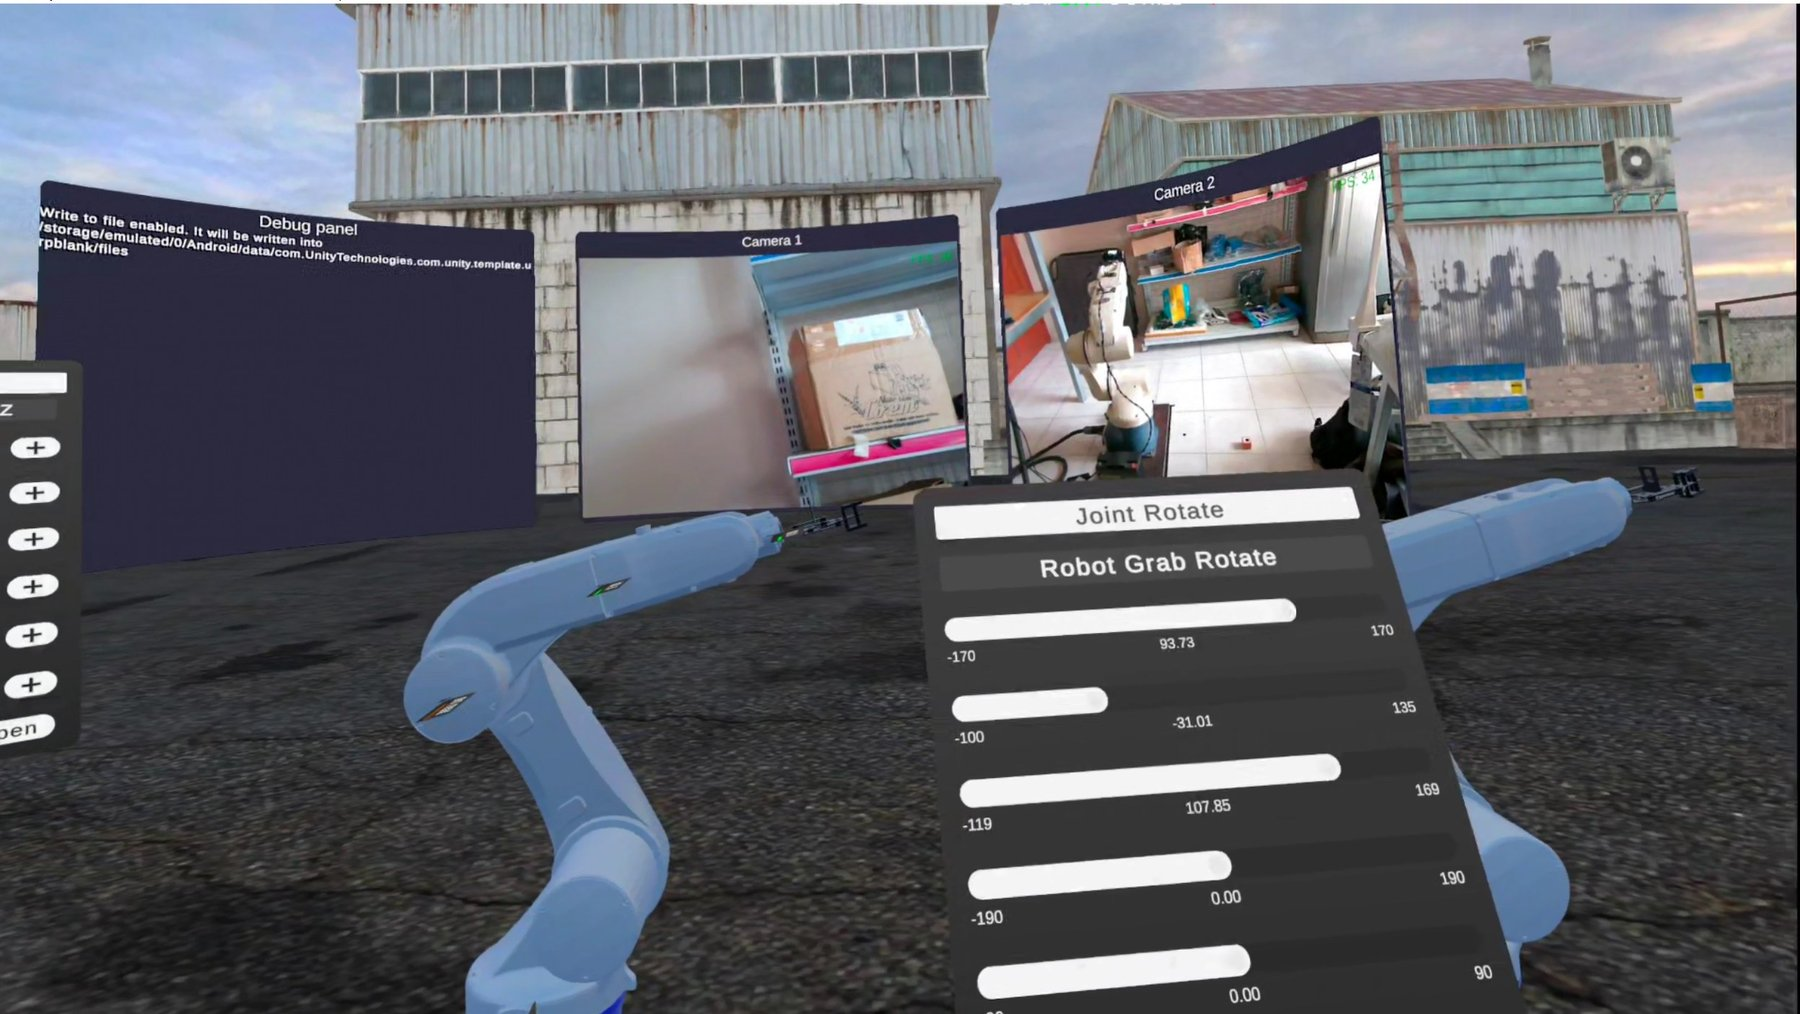
\includegraphics[width=0.8\linewidth]{Images/Implementation/vr_joint_rotate.jpg}
    \caption{Điều khiển cánh tay bằng slider trong ứng dụng VR}
    \label{fig:eval-vr-joint-rotate}
\end{figure}

\textbf{Điều khiển cánh tay robot thông qua tương tác với mô hình tương lai}

Nhấn nút "Robot Grab Rotate" để chuyển sang chế độ điều khiển thông qua việc tương tác (nắm vào kéo) mô hình 3D của cánh tay robot tương lai. Các trục đã được giới hạn để đảm bảo rằng góc kéo không vượt quá ngưỡng hoạt động thực tế của cánh tay robot. Ở phần slider, mỗi trục sẽ thể hiện màu để báo hiệu nếu trục gần đạt đến ngưỡng giới hạn.

Khi đã chỉnh hình dạng của cánh tay robot, nhấn nút Execute sẽ đưa cánh tay thực tế tới vị trí như đã tinh chỉnh.

\begin{figure}[H]
    \centering
    \begin{subfigure}{0.48\linewidth}
        \centering
        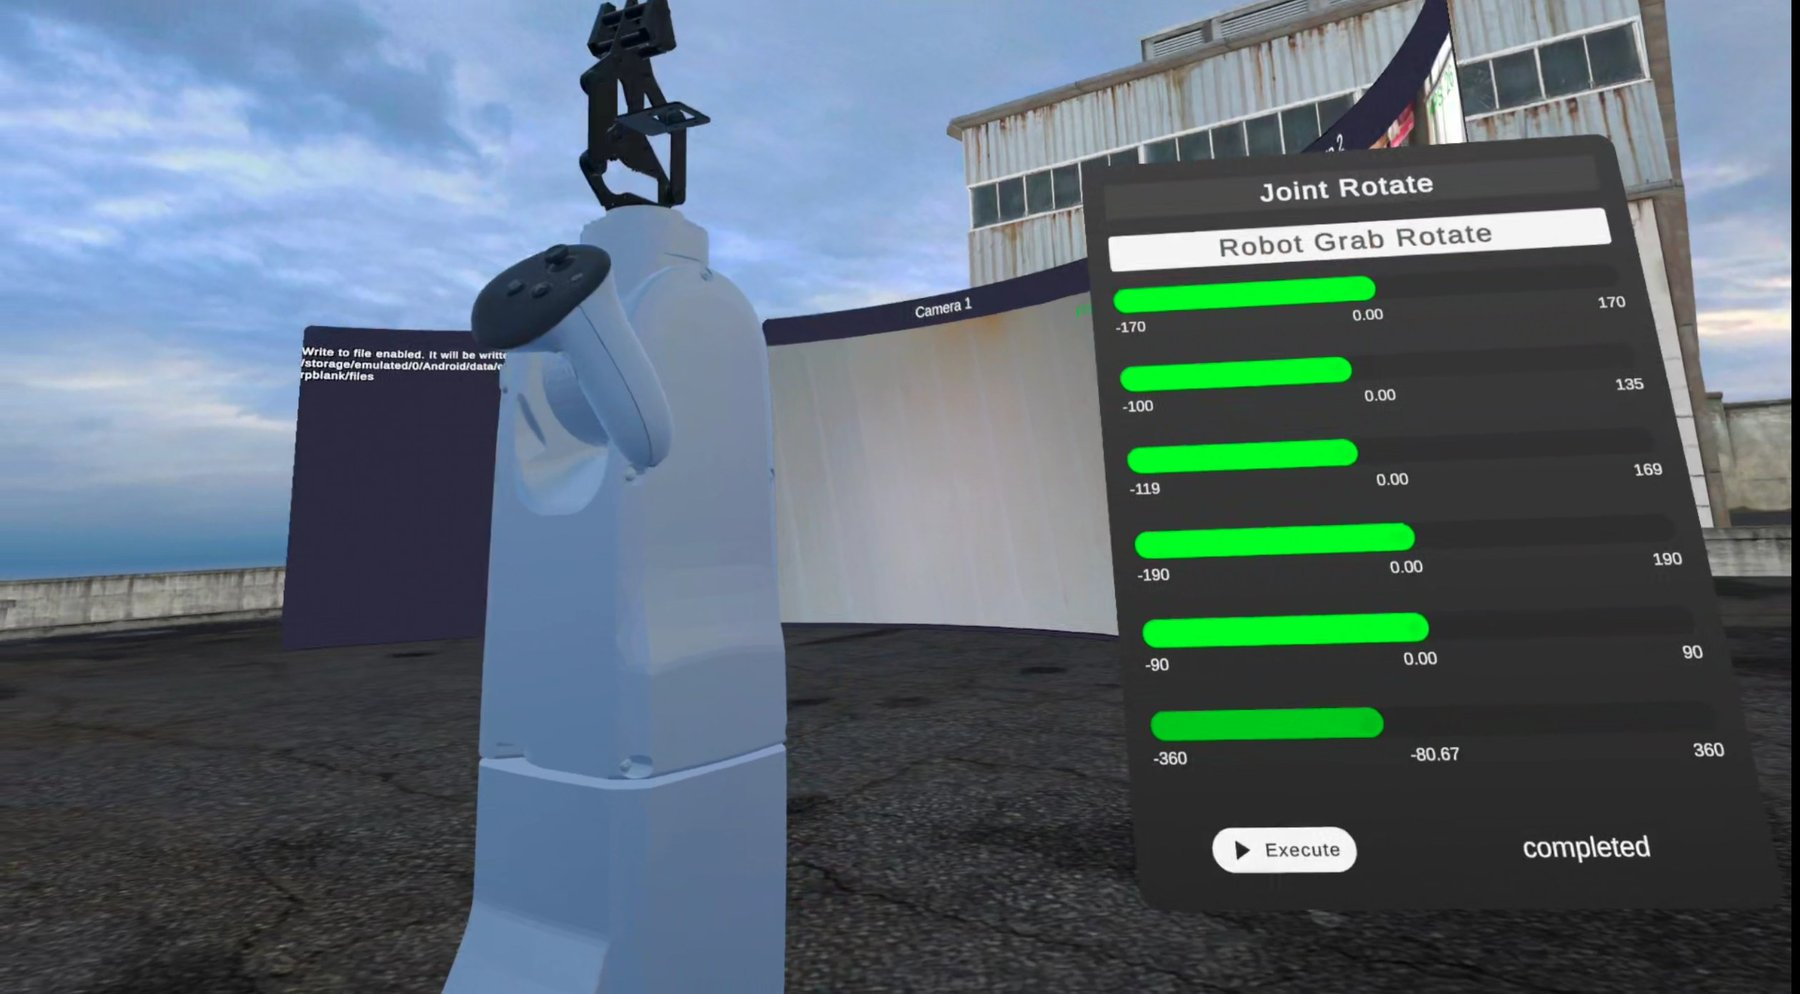
\includegraphics[width=\linewidth]{Images/Implementation/vr_grab_rotate.jpg}
        \caption{Giao diện Robot Grab Rotate}
    \end{subfigure}
    \hfill
    \begin{subfigure}{0.48\linewidth}
        \centering
        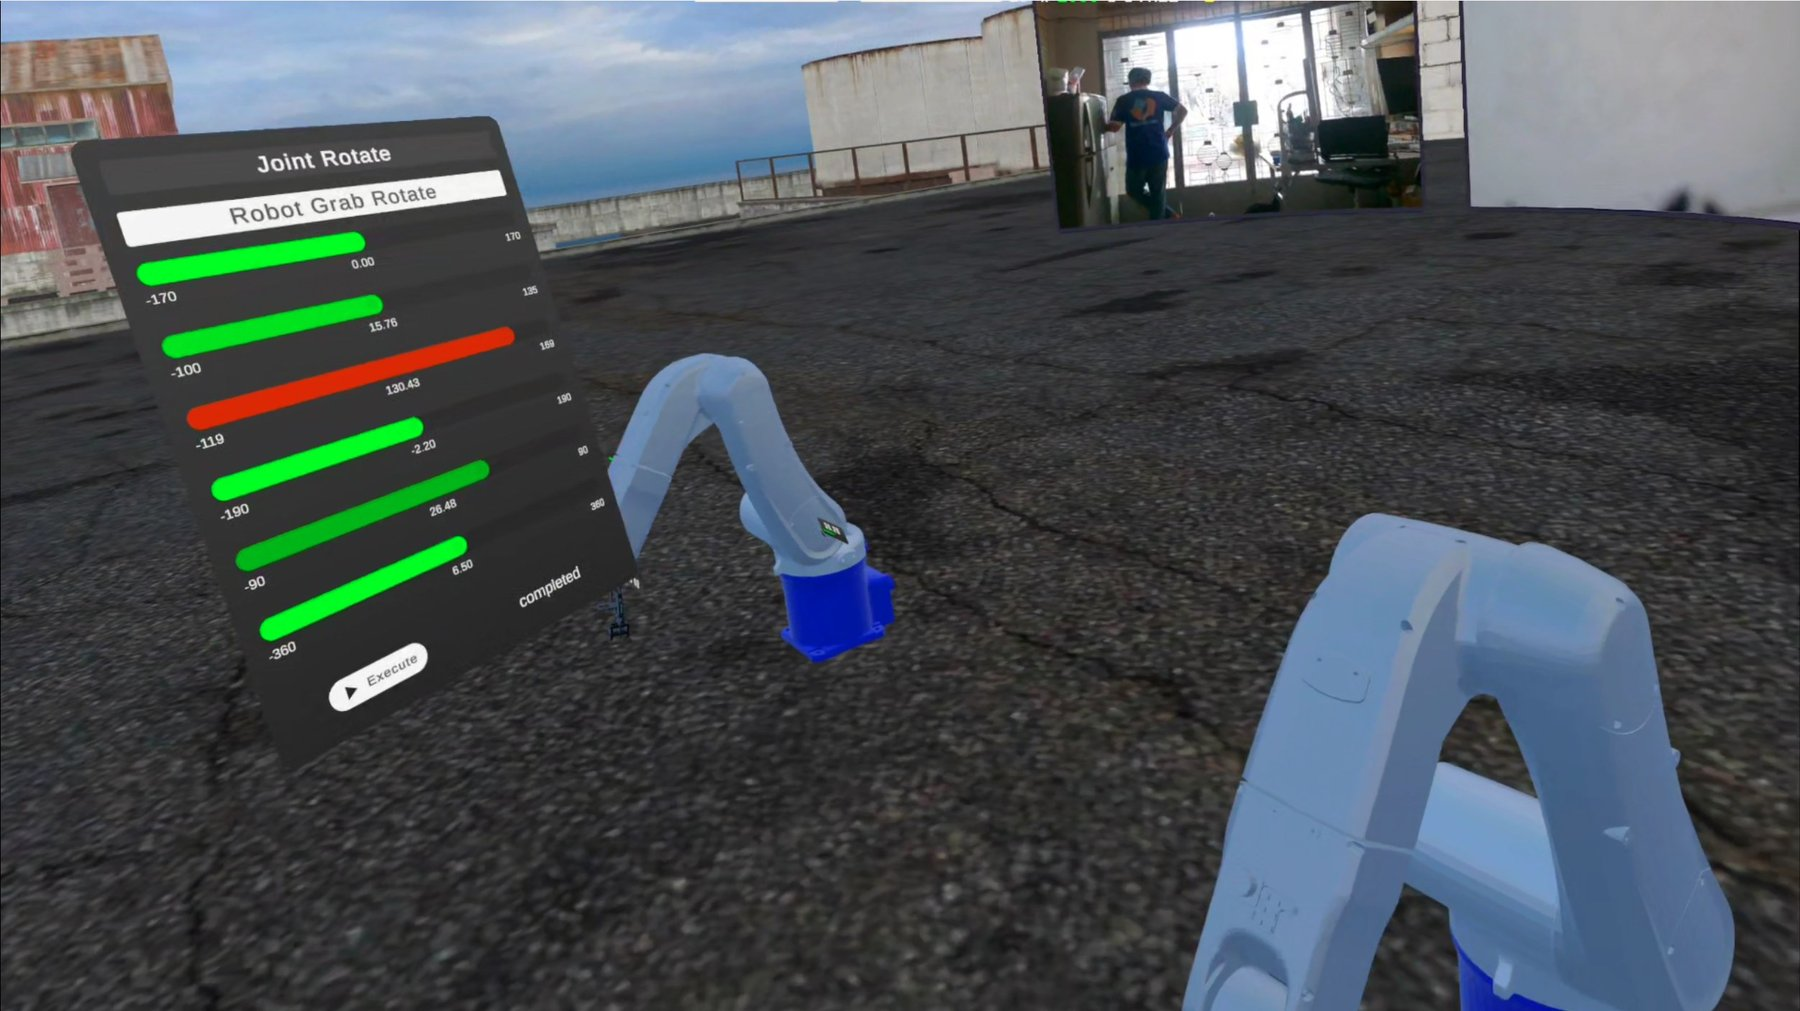
\includegraphics[width=\linewidth]{Images/Implementation/vr_grab_rotate_1.jpg}
        \caption{Thao tác xoay bằng tương tác trực tiếp}
    \end{subfigure}
    \caption{Điều khiển cánh tay bằng tương tác mô hình tương lai}
    \label{fig:eval-vr-grab-rotate}
\end{figure}

\subsubsection{Đánh giá độ trễ truyền nhận thông qua Ros-Sharp giữa ứng dụng và Ros2}

Độ trễ truyền nhận giữa ứng dụng VR và máy PC chạy Ros2 là tiêu chí quan trọng phản ánh mức độ đồng bộ giữa thao tác của người dùng trên kính VR và phản hồi từ hệ thống robot. Để đo đạc chỉ tiêu này, đề tài xây dựng một node Ros2 chuyên dụng (\texttt{topic\_latency\_benchmark}) thực hiện cơ chế ping-pong qua hai topic:

\begin{itemize}
    \item Node Ros2 (PC) publish một gói tin \texttt{std\_msgs/String} lên topic \texttt{/benchmark} mỗi 100\,ms. Payload của gói tin chứa timestamp gửi dưới dạng chuỗi số nanosecond (\texttt{rclcpp::Clock}) để định danh gói.
    \item Ứng dụng VR (Meta Quest~3) subscribe \texttt{/benchmark} thông qua Ros-Sharp/RosBridge WebSocket, sau khi nhận được gói tin, ngay lập tức publish phản hồi lên topic \texttt{/ack} với nội dung payload tương tự.
    \item Khi node Ros2 nhận được \texttt{/ack}, nó tính RTT bằng công thức: 
    
    $\text{RTT} = t_{\text{ack received}} - t_{\text{last benchmark publish}}$, 
    
    với $t$ là thời gian của ROS clock trên cùng máy PC.
\end{itemize}

Phép đo bao gồm toàn bộ đường đi: Ros2 --> ứng dụng VR --> Ros2. Đây là RTT thực tế của vòng giao tiếp điều khiển, chịu một phần ảnh hưởng của độ trễ mạng kết nối.

Để đánh giá khả năng chịu tải mạng, đề tài sử dụng công cụ \textbf{iperf} để mô phỏng băng thông tải cao trên cùng kết nối Wi-Fi. iperf là công cụ đo lường hiệu năng mạng mã nguồn mở, có khả năng tạo ra luồng lưu lượng UDP/TCP liên tục với băng thông tùy chỉnh. Lệnh sử dụng:

\begin{lstlisting}[style=bashstyle]
iperf -c 192.168.2.28 -u -b <x>M -t 0
\end{lstlisting}

Trong đó: \texttt{-c} chỉ định địa chỉ IP của server iperf (máy PC); \texttt{-u} sử dụng giao thức UDP; \texttt{-b <x>M} đặt băng thông mục tiêu \textit{x}\,Mbit/s; \texttt{-t 0} chạy liên tục cho đến khi dừng thủ công. Lệnh này được chạy từ một thiết bị khác trên cùng mạng Wi-Fi, tạo ra lưu lượng nền 100, 150 và 200\,Mbit/s để kiểm tra sự ổn định của kết nối VR--Ros2 khi băng thông bị tải cao. Kết quả đánh giá RTT theo từng điều kiện như sau:

% ── Tự động tạo bởi scripts/analyze_rtt_latency.py ──────────────────────
\begin{figure}[H]
\centering
\begin{tikzpicture}
\begin{axis}[
    ybar,
    width=0.88\linewidth,
    height=6cm,
    bar width=14pt,
    xlabel={Điều kiện tải mạng},
    ylabel={RTT (ms)},
    symbolic x coords={Bình thường, 100 Mbit/s, 150 Mbit/s, 200 Mbit/s},
    xtick=data,
    xticklabel style={font=\small},
    ymin=0, ymax=110,
    ytick={0,20,40,60,80,100},
    ymajorgrids=true,
    major grid style={line width=0.4pt, draw=gray!40},
    legend style={at={(0.98,0.98)}, anchor=north east, font=\small,
                  draw=gray!40, fill=white},
    legend cell align=left,
    axis lines=left,
    enlarge x limits=0.18,
]
% Trung bình (TB)
\addplot[fill=blue!60, draw=blue!80] coordinates {
    (Bình thường, 22.6)
    (100 Mbit/s, 27.4)
    (150 Mbit/s, 38.7)
    (200 Mbit/s, 50.2)
};
\addlegendentry{TB}
% P50 (Trung vị)
\addplot[fill=green!60, draw=green!80!black] coordinates {
    (Bình thường, 19.0)
    (100 Mbit/s, 23.5)
    (150 Mbit/s, 33.3)
    (200 Mbit/s, 52.8)
};
\addlegendentry{P50}
% P95
\addplot[fill=orange!70, draw=orange!90] coordinates {
    (Bình thường, 52.4)
    (100 Mbit/s, 58.3)
    (150 Mbit/s, 82.3)
    (200 Mbit/s, 93.4)
};
\addlegendentry{P95}
% P99
\addplot[fill=red!60, draw=red!80] coordinates {
    (Bình thường, 80.0)
    (100 Mbit/s, 88.0)
    (150 Mbit/s, 95.8)
    (200 Mbit/s, 98.1)
};
\addlegendentry{P99}
\end{axis}
\end{tikzpicture}
\caption{RTT (TB / P50 / P95 / P99) theo điều kiện tải mạng Wi-Fi giữa ứng dụng VR (Meta Quest~3) và Ros2 (PC)}
\label{fig:rtt-bar-chart}
\end{figure}

\begin{table}[H]
\centering
\caption{Thống kê RTT giữa ứng dụng VR và RosBridge WebSocket theo điều kiện tải mạng}
\label{tab:rtt-latency}
\small
\begin{tblr}{
    colspec = {|X[3.2,l]|X[1,c]|X[1.2,c]|X[1.2,c]|X[1.2,c]|X[1.2,c]|X[1.2,c]|X[1.2,c]|},
    hlines,
    row{1} = {font=\bfseries, bg=gray!20},
}
Điều kiện & $N$ & Min (ms) & TB (ms) & Trung vị (ms) & P95 (ms) & P99 (ms) & Max (ms) \\
Bình thường & 1426 & 0{,}8 & 22{,}6 & 19{,}0 & 52{,}4 & 80{,}0 & 97{,}3 \\
Tải cao 100\,Mbit/s & 1001 & 0{,}7 & 27{,}4 & 23{,}5 & 58{,}3 & 88{,}0 & 99{,}4 \\
Tải cao 150\,Mbit/s & 813 & 0{,}4 & 38{,}7 & 33{,}3 & 82{,}3 & 95{,}8 & 99{,}4 \\
Tải cao 200\,Mbit/s & 955 & 0{,}0 & 50{,}2 & 52{,}8 & 93{,}4 & 98{,}1 & 99{,}8 \\
\end{tblr}
\end{table}

Kết quả đo đạc RTT được trình bày tại Bảng~\ref{tab:rtt-latency} và Hình~\ref{fig:rtt-bar-chart}.

\textbf{Điều kiện mạng bình thường.}
Khi không có lưu lượng tải cao ($N = 1426$ mẫu), RTT trung bình đạt
\textbf{22{,}6\,ms} (trung vị 19{,}0\,ms), dao động từ 0{,}8\,ms đến 97{,}3\,ms
với độ lệch chuẩn 13{,}9\,ms.
P95 ở mức \textbf{52{,}4\,ms} và P99 ở mức \textbf{80{,}0\,ms} cho thấy phần lớn
các gói tin được truyền nhận trong vòng 50\,ms -- phù hợp với yêu cầu phản hồi
nhanh của ứng dụng điều khiển thời gian thực qua kính VR.

\textbf{Ảnh hưởng của tải mạng tải cao (iperf UDP).}
Khi áp lưu lượng nền 100\,Mbit/s bằng iperf, RTT trung bình tăng lên
\textbf{27{,}4\,ms} ($+$21{,}4\% so với điều kiện bình thường), P99 tăng lên 88{,}0\,ms.
Ở mức 150\,Mbit/s, RTT trung bình là \textbf{38{,}7\,ms} ($+$71{,}5\%),
và tại 200\,Mbit/s lên tới \textbf{50{,}2\,ms} ($+$122{,}3\%).
RTT tăng theo xu hướng gần tuyến tính với băng thông tải cao, nên để đảm bảo ứng dụng VR có thể giao tiếp hiệu quả với độ trễ thấp, độ lớn của dữ liệu truyền nhận cũng như tính chất của mạng cần được quan tâm.

\textbf{Nhận xét chung.}
Có thể thấy, độ trễ của giao tiếp giữa ứng dụng VR và Ros2 thông qua Ros-sharp vẫn chịu ảnh hưởng của tải mạng, với số liệu cho thấy thời gian RTT tăng dần khi tải mạng tăng cao. Thêm nữa, với việc sử dụng Ros-Sharp, cơ chế giao tiếp giữa ROS2 với kính VR vẫn là giao tiếp thông qua Web Socket (dạng TCP/IP), do đó chịu ảnh hưởng của cơ chế Head-of-line-blocking và nỗ lực truyền dữ liệu tin cậy, cho cả gói tin quan trọng (như /joint\_states) và dữ liệu ảnh lớn (image\_raw), nên sẽ gặp vấn đề nếu lượng dữ liệu truyền đi tăng thêm hoặc mạng bị chập chờn. Để tăng tính hiệu quả của giao tiếp, phương thức giao tiếp sử dụng UDP nên được cân nhắc, có thể thay thế sử dụng Web Socket bằng WebRTC (cho phép tách biệt truyền gói tin dạng UDP cho dữ liệu camera/ cloud sensor, hoặc dữ liệu quan trọng thì sử dụng TCP) với \href{https://docs.phntm.io/bridge/}{Phantom bridge}, và bên phía Unity sẽ phát triển bộ kết nối/ giao tiếp sử dụng WebRTC, trao đổi dữ liệu theo giao thức \href{https://github.com/RobotWebTools/rosbridge_suite/blob/ros2/ROSBRIDGE_PROTOCOL.md#422-default-qos-settings}{RosBridge Protocol V2} để phù hợp theo yêu cầu của Ros2.

Trong đề tài hiện tại, với lợi thế của mạng Wifi cục bộ và việc xây dựng ứng dụng ROS2 sử dụng C++, độ trễ giữa ứng dụng VR và ROS2 rơi vào khoảng 20ms trong điều kiện sử dụng bình thường, qua đó giúp cho việc truyền dữ liệu hình ảnh cũng như đồng bộ trạng thái hoạt động trong 10ms. 

\subsubsection{Đánh giá hiệu năng ứng dụng trong quá trình hoạt động}

Một trong những vấn đề trong việc phát triển ứng dụng VR đó là đảm bảo người dùng có trải nghiệm sử dụng mượt mà, thoải mái mà không gây gánh nặng nhận thức (cognitive pressure). Meta Quest Developer Hub được sử dụng để thu thập chi tiết dữ liệu hoạt động của ứng dụng, gồm nhiều tiêu chí đánh giá khác nhau để xem xét ứng dụng có đang hoạt động ổn định và tối ưu hay không. Bảng phân tích các tiêu chí và nhận xét được thể hiện ở dưới:

Dữ liệu được thu thập qua 1 phiên sử dụng ứng dụng liên tục (tổng cộng
27{,}3\,phút) bằng Meta Quest Developer Hub trên thiết bị Meta Quest 3.
Bảng~\ref{tab:vr-app-metrics} trình bày các tiêu chí hiệu năng chính được ghi nhận
trong suốt quá trình hoạt động.

\begin{table}[H]
\centering
\caption{Tổng hợp hiệu năng ứng dụng VR trên Meta Quest~3 (1 phiên đo, tổng 27{,}3 phút)}
\label{tab:vr-app-metrics}
\small
\begin{tblr}{
    colspec = {|X[4.2,l]|X[1.1,c]|X[1.2,c]|X[1.2,c]|X[1.2,c]|X[1.6,c]|},
    hlines,
    row{1}  = {font=\bfseries, bg=gray!20},
    row{2}  = {bg=gray!10, font=\itshape},
    row{8}  = {bg=gray!10, font=\itshape},
    row{11} = {bg=gray!10, font=\itshape},
    row{14} = {bg=gray!10, font=\itshape},
    row{18} = {bg=gray!10, font=\itshape},
}
Tiêu chí & Đơn vị & TB & Min & Max & Mục tiêu \\
\SetCell[c=6]{l} \textit{Hiệu năng khung hình} \\
FPS trung bình & fps & 72{,}0 & 62 & 73 & $\geq$72 \\
GPU render time / frame & ms & 8{,}60 & 5{,}95 & 11{,}03 & $\leq$13{,}9 \\
ATW GPU time / frame & ms & 1{,}56 & 1{,}12 & 3{,}31 & nhỏ \\
\SetCell[c=6]{l} \textit{Tải CPU / GPU} \\
CPU utilization (tổng 8 nhân) & \% & 52{,}8 & 35 & 69 & $<$80 \\
GPU utilization & \% & 75{,}1 & 55 & 83 & $<$80 \\
Tần số CPU & MHz & 1511 & 1228 & 2361 & -- \\
\SetCell[c=6]{l} \textit{Bộ nhớ} \\
RAM ứng dụng (PSS) & MB & 1010{,}7 & 940 & 1038 & -- \\
GPU memory vật lý & MB & 344{,}2 & 335 & 346 & -- \\
\SetCell[c=6]{l} \textit{Ổn định khung hình (tổng 2 phiên)} \\
Stale frames & frames & \SetCell[c=4]{c} 4307 & & & 0 \\
Skipped frames (ATW miss) & frames & \SetCell[c=4]{c} 0 & & & 0 \\
Shader hitches & lần & \SetCell[c=4]{c} 0 & & & 0 \\
\SetCell[c=6]{l} \textit{Nhiệt độ thiết bị} \\
Nhiệt độ pin & \textdegree{}C & 46{,}3 & 43 & 47 & $<$45 \\
\end{tblr}
\end{table}

\textbf{Khung hình và độ trễ hiển thị.}

\textit{FPS ứng dụng} là số khung hình Unity render được mỗi giây, phản ánh trực tiếp
trải nghiệm mượt mà của người dùng trong môi trường VR. Theo yêu cầu VRC.Quest.Performance.1
của Meta \cite{meta_vrc_performance}, ứng dụng phải duy trì tối thiểu \textbf{60\,fps} liên tục
trong suốt phiên sử dụng; mục tiêu lý tưởng với Meta Quest~3 cấu hình mặc định là bám sát
\textbf{72\,fps} (refresh rate của màn hình). FPS dưới 60 kéo dài gây hiện tượng giật và
tăng nguy cơ say chuyển động (motion sickness). Ứng dụng đạt trung bình \textbf{72{,}0\,fps}
(min 62, max 73), bám sát ngưỡng 72\,fps trong phần lớn phiên sử dụng -- cải thiện đáng kể
so với các phiên đo trước đây.

\textit{GPU render time / frame} (App GPU Time) là thời gian GPU hoàn thành toàn bộ công việc
đồ hoạ cho một frame. Đây là chỉ số then chốt để xác định ứng dụng đang bị bottleneck tại
CPU hay GPU \cite{meta_ovr_best_practices}. Ngân sách frame phụ thuộc vào refresh rate mục
tiêu: tại 72\,Hz là \textbf{13{,}88\,ms}, tại 90\,Hz là 11{,}11\,ms và tại 120\,Hz là
8{,}33\,ms. Nếu App GPU Time vượt ngân sách, ứng dụng bị GPU-bound; ngược lại nếu App GPU
Time thấp nhưng FPS vẫn không đạt, ứng dụng bị CPU-bound. Giá trị đo được \textbf{8{,}60\,ms}
trung bình -- khoảng 62\% ngân sách -- cho thấy pipeline render còn dư headroom; kết hợp với
GPU utilization trung bình 75\%, GPU đang trở thành nút cổ chai chính.

\textit{ATW GPU time / frame} (TimeWarp GPU Time) là thời gian GPU dành riêng cho cơ chế
Asynchronous TimeWarp (ATW) ở tầng compositor của Horizon OS. ATW chạy hoàn toàn độc lập
với ứng dụng: khi ứng dụng không kịp nộp frame đúng hạn, ATW tổng hợp frame trung gian
bằng cách biến đổi frame cũ nhất theo dữ liệu chuyển động đầu mới nhất, duy trì refresh
rate hiển thị. Chỉ số này cần giữ ở mức thấp để không tranh chấp GPU headroom với app;
đỉnh quá cao có thể dẫn tới screen tear \cite{meta_ovr_stats}. Ứng dụng đạt
\textbf{1{,}56\,ms} trung bình (đỉnh 3{,}31\,ms), ở mức an toàn và không cạnh tranh với
App GPU Time.

\textbf{Tải CPU và GPU.}

\textit{CPU utilization} ở đây là tổng mức sử dụng CPU trên cả 8 nhân của SoC Snapdragon
XR2 Gen~2. Cần lưu ý rằng chỉ số này không phân biệt luồng render với các luồng khác
(Ros-Sharp, networking, IK). Mức tải dưới \textbf{80\%} được khuyến nghị để tránh scheduling
pressure ảnh hưởng tới deadline renderer \cite{meta_ovr_stats}; trên 90\% kéo dài sẽ bắt
đầu gây stale frame. Ứng dụng đạt \textbf{52{,}8\%} trung bình với đỉnh \textbf{69\%},
còn dư headroom tốt. CPU không còn là nút cổ chai trong phiên này, nhờ một số cải thiện sau:

\begin{itemize}
    \item \textbf{Tắt mipmaps*}: Trong hàm xử lý ảnh của \textbf{CompressedImageSubscriber}, Texture2D Apply dữ liệu ảnh với tham số \textbf{updateMipmaps = false} và makeNoLongerReadable = false. "Mipmaps" là một khái niệm trong Unity, có vai trò tạo ra nhiều mức độ ảnh (level) cho một đối tượng, và hỗ trợ tự động chọn độ phân giải của đối tượng đó tùy theo khoảng cách với camera. Nếu Camera gần, thì mức độ chi tiết ảnh của đối tượng sẽ giữ chất lượng gốc, nhưng càng ra xa, thì sẽ sử dụng level 1 (nửa độ phân giải), level 2 (1/4 độ phân giải)... Điều này giúp cho game tiết kiệm đáng kể chi phí render hình ảnh đối tượng, giảm tải cho GPU. Tuy nhiên, cơ chế này chỉ phù hợp cho một đối tượng với hình ảnh cố định. Đối với hình ảnh từ camera liên tục thay đổi (30FPS), tính năng này khiến cho Mipmaps bị tính lại liên tục, gây một lượng tải rất lớn cho CPU. Ngoài ra, ảnh camera cũng chỉ được hiển thị trên UI canvas, trên một mặt phẳng, nên việc sử dụng cơ chế Mipmaps là không cần thiết. 
    \item \textbf{Giãn cách lệnh Publish cho MoveIt-Servo control}: Khi nhấn nút xoay robot bằng MoveIt-Servo, hàm được thiết kế ban đầu là gửi lệnh publish liên tục theo framerate. Tuy nhiên, với ~72fps, lệnh publish được gửi với tần số nhanh (13.66ms / 1 lần publish). Điều này vô tình tăng tải xử lý cho CPU để thực hiện publish tới ROS, trong khi đó MoveIt-Servo được cấu hình là chỉ dừng xoay khi lệnh tới trễ hơn 300ms. Do đó, các lớp (Class) Publish vào MoveIt-Servo sẽ chỉ gửi đi mỗi 100ms thay vì mỗi frame, giúp giảm đáng kể tải CPU phải xử lý.
\end{itemize}

\textit{GPU utilization} là mức sử dụng GPU tổng thể của ứng dụng. Ngưỡng
dưới \textbf{80\%} là bình thường; từ 80--90\% bắt đầu có rủi ro scheduling GPU gây frame
drop; 100\% kéo dài nghĩa là GPU-bound hoàn toàn \cite{meta_ovr_stats}. Ứng dụng đạt
\textbf{75{,}1\%} trung bình (đỉnh 83\%), tiệm cận ngưỡng an toàn 80\%. Chỉ số này
nhất quán với App GPU Time ở mức 8{,}60\,ms (62\% ngân sách) và xác nhận GPU hiện là
nút cổ chai chính; đỉnh 83\% cho thấy cần tối ưu hóa draw call và shader để tránh frame drop. Tuy vậy, đây vẫn là một mức tiêu thụ GPU chấp nhận được, và cho ra kết quả hoạt động ứng dụng có FPS trung bình nằm ở mức 72FPS.

\textit{Tần số CPU} phản ánh cơ chế DVFS (Dynamic Voltage and Frequency Scaling) của SoC:
xung tăng tự động khi tải cao và giảm khi nhiệt độ tiệm cận ngưỡng throttle nhiệt. Tần số
dao động từ \textbf{1228\,MHz} đến \textbf{2361\,MHz} trong suốt phiên, cho thấy hệ thống
boost clock khi cần nhưng chưa xảy ra throttle (nếu throttle, tần số sẽ tụt đột ngột
xuống dưới mức nền và kèm theo FPS giảm bất thường).

\textbf{Bộ nhớ.}

\textit{RAM ứng dụng (PSS -- Proportional Set Size)} là dấu chân bộ nhớ RAM thực tế của
tiến trình, trong đó các vùng nhớ chia sẻ với tiến trình khác chỉ được tính theo tỉ lệ sử
dụng. PSS chính xác hơn RSS (Resident Set Size) vì tránh đếm trùng bộ nhớ chia sẻ, đây là
chỉ số chuẩn Android để theo dõi footprint thực \cite{android_memory_overview}. Giá trị
\textbf{1010{,}7\,MB} trung bình (đỉnh 1038\,MB) ổn định, không tăng tuyến tính theo thời gian,
không có dấu hiệu memory leak -- chứng tỏ Unity đang giải phóng Texture2D từ luồng ảnh
camera và các object tạm đúng cách. Mức PSS cao hơn so với báo cáo trước đó là do bật tính năng Development Build (để theo dõi hiệu năng ứng dụng và hỗ trợ Profiling) cùng Immersive Debugging (một tính năng đặc biệt dành cho thiết bị Meta Quest, cho phép hiển thị bảng Debug Log của Unity ngay trong ứng dụng).

\textit{GPU memory vật lý} là phần bộ nhớ đồ hoạ thực tế ứng dụng chiếm dụng cho
texture, framebuffer, mesh buffer và shader. Giá trị \textbf{344{,}2\,MB} trung bình (đỉnh
346\,MB) ổn định, phản ánh asset 3D của cánh tay robot Denso cùng các shader được tải vào
VRAM một lần và giữ xuyên suốt phiên, không có spike lớn do texture streaming bất thường.

\textbf{Ổn định khung hình.}

\textit{Stale frames} là số lần compositor đã sẵn sàng hiển thị frame mới nhưng ứng dụng
chưa nộp frame đúng hạn, khiến compositor phải dùng lại frame cũ và nhờ ATW bù chuyển động.
Khác với skipped frame, stale frame vẫn được hiển thị nhờ ATW nhưng nội dung scene chưa
được cập nhật -- người dùng có thể nhận thấy lag nhỏ giữa chuyển động đầu và phản hồi
hình ảnh \cite{meta_ovr_stats}. \textbf{4307 stale frames} trong 27{,}3 phút
($\approx$2{,}6/giây) -- giảm hơn 75\% so với phiên đo trước (17\,059 stale frames),
phản ánh cải thiện rõ rệt sau khi tối ưu hoá luồng điều khiển. Stale frame còn lại chủ yếu
xuất hiện tại các thời điểm GPU utilization đạt đỉnh 83\%; hướng cải thiện tiếp theo là
tối ưu GPU load để đưa stale frame về gần 0.

\textit{Skipped frames (ATW miss)} là số frame bị compositor bỏ qua hoàn toàn -- tức kể
cả ATW cũng không kịp tổng hợp frame trước deadline scan-out của màn hình. Đây là tình
huống nghiêm trọng nhất: người dùng thấy hình ảnh bị đứng/nhảy cóc, đây là nguyên nhân
hàng đầu gây motion sickness. Mục tiêu cứng của Meta là \textbf{0 skipped frame}
\cite{meta_ovr_stats}. Kết quả đo được \textbf{0 skipped frames} trong toàn phiên
là lý tưởng, xác nhận ATW GPU time (1{,}56\,ms) đủ thấp để compositor luôn hoàn thành
trước deadline dù ứng dụng có bị stale.

\textit{Shader hitches} là số lần Unity phải compile shader lúc runtime (pipeline
compilation stall), gây frame drop đột ngột thường thấy ở lần chạy đầu sau cài đặt khi
shader cache còn trống. Sau khi shader được compile và cache lại, hitches không còn xuất
hiện ở các phiên tiếp theo \cite{meta_ovr_best_practices}. \textbf{0 shader hitches} trong
phiên đo xác nhận shader đã được warm-up đúng cách trước khi thu thập dữ liệu (theo như Meta Quest, để đánh giá chính xác hiệu năng ứng dụng, sẽ cần phải khởi động ứng dụng lần đầu tiên để compile toàn bộ shader, sau đó mới tiến hành đo đạc).

\textbf{Nhiệt độ thiết bị.}

\textit{Nhiệt độ pin} là chỉ báo gián tiếp về nguy cơ thermal throttle của headset. Meta
Quest 3 có ba power state do Horizon OS quản lý \cite{meta_ovr_stats}: \textbf{NORMAL} (hoạt
động bình thường), \textbf{SAVE} (giảm xung CPU/GPU để tản nhiệt, khoảng \textasciitilde45--50\,°C
tuỳ cảm biến), và \textbf{DANGER} (hiển thị cảnh báo quá nhiệt và buộc giảm hiệu năng
nghiêm trọng, khoảng \textasciitilde53\,°C). Khi vào SAVE, FPS và chất lượng render bị
giảm tự động dù ứng dụng không thay đổi. Nhiệt độ pin đo được \textbf{46{,}3\,°C} trung
bình (đỉnh 47\,°C) vượt nhẹ mức 45\,°C Meta khuyến nghị cho trải nghiệm thoải mái nhưng
chưa đạt ngưỡng SAVE hay DANGER. Thiết bị duy trì ổn định ở power state NORMAL trong suốt
phiên 27{,}3 phút;



